\documentclass[sn-mathphys]{sn-jnl}
\usepackage[utf8]{inputenc}
%\usepackage{cite}
\usepackage{amsmath,amssymb,amsfonts}
\usepackage{algorithmicx}
\usepackage{algpseudocode}
\usepackage{graphicx}
\usepackage{textcomp}
\usepackage{xcolor}
\usepackage[normalem]{ulem}
\usepackage{enumitem}
\usepackage{fancyvrb}
\usepackage{url}
%\usepackage[hidelinks,breaklinks]{hyperref}
\usepackage{booktabs}
\usepackage{multirow}
\usepackage{lscape}
\usepackage{listings}
\usepackage{rotating}
\usepackage{titlesec}
\titleformat*{\subsubsection}{\em}
\newcommand{\vthierry}[1]{{\color{magenta} @vthierry:[#1]}}
\newcommand{\chloe}[1]{{\color{blue} @chloe:[#1]}}
%\newcommand{\fred}[1]{{\color{red} @fred:[#1]}}
\newcommand{\defq}{\stackrel {\rm def}{=}}
\newcommand{\tab}{\hphantom{~}}
\newcommand{\drawn}{\stackrel {\text{drawn}}{=}}
\newcommand{\eqline}[1]{~\vspace{0.1cm}\\\centerline{$#1$}\vspace{0.1cm}\\}
\newcommand{\hhref}[1]{\href{#1}{#1}}

\makeatletter
\renewcommand\tableofcontents{%
    \@starttoc{toc}%
}
\makeatother
%+ Fin onto2spa
\begin{document}

\title[Where is Aristotle in our brain?]{Where is Aristotle in our brain? On biologically plausible reasoning embedded in neuronal computation}
\author[1]{\fnm{Chloé} \sur{Mercier}}\email{chloe.mercier@inria.fr}
\author[1,2]{\fnm{Thierry} \sur{Viéville}}\email{thierry.vieville@inria.fr}
\equalcont{Supported by \href{Inria, AEx AIDE}{https://team.inria.fr/mnemosyne/en/aide}.}
\affil[1]{Mnemosyne Team, Inria Bordeaux, U. Bordeaux, LaBRI and IMN}
\affil[2]{LINE Laboratory, U. Côte d'Azur}

\abstract{

Human cognition involves tightly interleaved numerical but also symbolic (including logical) computations. Determining how the brain can implement such processing is an important issue, and we would like to address some aspects of this issue here by combining two approaches.

On the one hand, ontology-oriented languages allow us to describe symbolic structured knowledge and perform logical inference using entailment rules. To what extent this could provide a rather natural representation of usual human reasoning is an open question that we are going to discuss here, considering a generalization to modal logic; we will also go beyond deductive reasoning, discussing whether this could also apply to inductive and abductive reasoning.

On the other hand, spiking neuronal networks are biologically plausible implementations of brain circuit computations, meaning that they can provide a way to manipulate symbols embedded as numeric vectors that carry semantic information. In the present work, we consider such an architecture with the vector symbolic architecture (VSA) formalism, allowing us to describe neuronal implementations at an algebraic level.

This development illustrates how the former cognitive mechanisms can naturally emerge from distributed calculus, yielding neuro-symbolic computations. Our aim is to show that it can be implemented, considering a VSA approach, in biological neuronal computations. Such neuro-symbolic deductive mechanisms are especially useful in complex problem-solving.
}

\keywords{Ontology, Modal Logic, Semantic Pointer Architecture, Abstract Thought, Neuro-symbolism, Problem Solving.}

\maketitle

\vthierry{
\\- {See reviewer comments and anwers \href{here}{https://drive.google.com/drive/folders/1OfmsclVnMbaGDsC2560BsX8CyzXxooew}.}
\\- {For the review purpose, table of contents:} \\ {\tiny \tableofcontents}
}

\section{Introduction}

\subsection{From sensorimotor processing to logical reasoning}

It is generally admitted (as reviewed, e.g., in \cite{ness_knowledge_2007}) that human logical reasoning emerges progressively from the sensorimotor association, with the formation of stable concepts, even at a symbolic level, before it is possible to manipulate them at a concrete level, by performing inductive reasoning, and perform more formal deductive reasoning. Furthermore, as pointed out in \cite{arnett_adolescence_2001}, such a mechanism includes a cultural bias, since not all cultures feel the need to develop formal logical operation competencies, and obviously, most people do not use such formal operations in all aspects of their lives. However, as discussed in, e.g., \cite{keefer_metaphor_2016}, deductive reasoning, especially for goal-driven behavior, is deeply interleaved with heuristic deduction, which involves analogy and metaphor. Furthermore, as thoroughly studied by, e.g., \cite{purves_interplay_2001}, the experience of conscious or subconscious emotion has a powerful influence on rational decisions, including the choice of alternatives in deductive reasoning. Does this mean that the human brain does {\em not} need to develop deductive reasoning, except for singular cultural needs (e.g., for scholarship or to practice formal science)? Our understanding is that the situation is not binary. We need to make deductions to solve problems in everyday life, while the elements we briefly reviewed here demonstrate that such deductions are not Boolean (either true or false) but related to a given context, weighted by a certain level of belief, and biased by motivational elements in a wide sense.

In this study, we attempt to reconcile deductive reasoning with such cognitive mechanisms of inference to reach a biologically plausible neuronal implementation and show to what extent this could be extended to approximate deductive reasoning, in addition to inductive and abductive reasoning mechanisms\footnote{Here we make the distinction between
\\- {\em deductive reasoning}, which is the process of determining the formal logical consequence of some assumptions considered as true or approximately true;
\\- {\em inductive reasoning}, which is the process of inferring some general principle from a set of knowledge and plausible induction rules; and
\\- {\em abductive reasoning}, which is the process of inferring an explanation of some assertions, i.e., hypothesizing the precondition of a consequence.}.

Taking this discussion a step further, how does the brain give meaning to the symbols considered here? We will not address this issue here but would like to clarify some points. First of all, in neuro-symbolic studies, as reviewed in \cite{garcez_neurosymbolic_2020}, grounding is understood as the process of embedding symbolic computations onto real-valued features \cite{badreddine_logic_2021} because it provides a semantic interpretation or model (in the sense of a model of a set of logical assertions) of the symbolic system. This means that it is no longer an abstract set of assessments (potentially without any concrete implementation) but something that corresponds to a real formal object. 
Our approach thus does not solve the grounding problem, but in some sense, it does solve what we can call the ``anchoring'' problem of relating symbols to the neural substrate. This will be further discussed in the last section after the present approach is described in detail.


\subsection{Representing neuronal activity at a symbolic level}

As a possible entry point to considering a biologically plausible implementation at a symbolic level, vector symbolic architectures (VSAs) were introduced as a way to manipulate symbolic information represented as numeric vectors (see, e.g., \cite{levy_vector_2008} for an introduction). VSAs have been proven to be helpful in modeling high-level cognition and accounting for multiple biological features \cite{gayler_vector_2003,eliasmith_how_2013}. More specifically, the semantic pointer architecture (SPA) \cite{eliasmith_how_2013} instantiates so-called semantic pointers (i.e., vectors that carry semantic information) and makes it possible to manipulate them in networks of spiking neurons. This approach takes a significant step towards the unification of symbolic and sub-symbolic processing in that it provides a way to translate the former into the latter. Consequently, complex knowledge representations in the form of compositional structures that are traditionally restricted to symbolic approaches can now be distilled in numerical and even neural\footnote{The term ``neural" refers to any type of nerve cell, whereas ``neuronal" is specifically related to neurons.} systems \cite{crawford_biologically_2016}.

How can we represent a symbol in a neuronal assembly? A localist representation (one neuron or neuron group represented by a symbol) does not correspond to what is observed in the brain, and the basic idea is that a symbol corresponds to a pattern of activity of the whole assembly. Let us consider a spiking neuron network and quantify its activity using some statistics, e.g., the neuron rates or higher-order statistics (see, e.g., \cite{cessac_dynamics_2008} for a discussion). As developed in \cite{eliasmith_neural_2002}, this includes timing codes and population codes (i.e., relative timing codes between neurons), and the authors of \cite{eliasmith_neural_2002} show how, with their developed neural engineering framework (NEF), we can collect this high-dimensional set of bounded quantitative values, which can be normalized, as a unitary stochastic vector in a high-dimensional space (with a few thousand dimensions for a biological neuronal map and often a few hundred dimensions at the simulation level), defining a SPA. This includes a time representation in spiking neuron systems, not just a rate representation. The key point is that compared to other representations, e.g., based on synchrony within the neural assembly, the NEF alternative is much more scalable.

In the present study, we consider these developments as prerequisites and will simply consider that neural assembly activity is represented by a high-dimensional unary stochastic vector. We also need to specify transformations and define them at this abstract algebraic level. Mainly, following \cite{mercier_ontology_2021}, we will consider the auto-association mechanism, as developed in \cite{stewart_biologically_2011}, and functional transformations, as detailed in \cite{eliasmith_neural_2002}; their development is based, in a nutshell, on parameterized kernel-based approaches.

\subsection{What is this paper about?}

We first revisit how to encode symbols within the VSA approach based on the framework introduced in \cite{eliasmith_how_2013}, analyzing in more detail than previous works the numerical approximation statistic, because this is needed to model the VSA mechanism at a macroscopic level. We also describe how to generalize symbol encoding considering a related degree of belief, beyond binary information, and following \cite{mercier_ontology_2021}, we explain the semantic interest of such a generalization.

We then consider knowledge hierarchical structure encoding in the sense of, e.g., \cite{eichenbaum_memory_2017}, as a complement to associative and sequential memorization, and we discuss how to implement such a memory structure using the VSA. To this end, we have to review VSA data structures and demonstrate that they are linked to cognitive memory classification according to \cite{eichenbaum_memory_2017}. To better understand their computational properties, we also illustrate how such existing VSA data structures compare to programming language containers. 

This new data structure is the basic tool that is used to then study to what extent symbolic inference could be implemented by specific connectivity feedback, and, as a second contribution, we show that the vanilla fixed-point algorithm used for a forward deduction on a decidable set of entailment rules can be adapted to this biologically plausible framework, making it possible to perform deductive reasoning and also, to some extent, inductive and abductive reasoning.

We finally illustrate the proposed mechanism using both a simulation at the mesoscopic level, utilizing the well-established Nengo simulator, and also a simulation at the macroscopic scale. We show, as the third contribution of this paper, that such computations may be, up to a certain point, approximated without explicitly performing computations at the vector component level; instead, an algorithmic ersatz can be used.


\section{Symbolic information encoding} \label{encoding}

\subsection{Symbol encoding} \label{symbol-encoding}

At the numerical level, each symbol is implemented as a randomly drawn fixed unit $d$-dimensional vector $\mathbf{x} \in {\mathcal R}^d$. Typically, $d\simeq 100 \cdots 1000$, and we expect to manipulate $k\simeq 100 \cdots 10000$ symbols at the simulation level. A typical dimension of $256$ has been considered in related studies, such as \cite{mercier_ontology_2021}. Here, our macroscopic implementation uses the same dimension. In a cortical or brain map, the order of magnitude is higher since the vector corresponds to the neuronal map activity (thus it is closer to $10^{5\cdots 6}$) and the number of encoded symbols depends on which map is considered.

The vector components are drawn from a normal distribution ${\mathcal N}(0, \sigma^2)$, i.e., this distribution has zero mean and a standard deviation $\sigma \deq 1/\sqrt{d}$, in order to have an average magnitude of $1$.

A similarity measure is now introduced in order to semantically compare two vectors. This precisely means that both vectors\footnote{Let us consider two vectors ${v}_1 = {\bf u} + {\bf w}_1$ and ${v}_2 = {\bf u} + {\bf w}_2$ thus carrying the same semantic information encoded in ${\bf u}$ plus, say other independent information ${\bf w}_1$ and ${\bf w}_2$ independent from ${\bf u}$ and form each other. Then ${v}_1^T {v}_2 = {u}^T {u} = 1$, since other vectors orthogonal. This is the precise meaning of semantic similarity.} in and carries similar information. Classically, the cosine similarity (i.e., normalized dot product, denoted $\cdot$) is used to compute the semantic similarity between two unit vectors:
\eqline{\mathbf{x} \cdot \mathbf{y} \defq \mathbf{x}^\top \mathbf{y} = \cos\left(\widehat{\mathbf{x}, \mathbf{y}}\right),}
where $\mathbf{x}^\top$ denotes the transpose of $\mathbf{x}$.  This measure obviously corresponds to the angular distance between the vectors.

The key property is that, provided that the space dimension $d$ is large enough, two randomly chosen different vectors will be approximately orthogonal. More precisely,
\eqline{{\bf x} \cdot {\bf y} \sim \delta_{{\bf x} = {\bf y}} + {\mathcal N}(0, 1/d),}
i.e., it is almost $1$ if equal and $0$ otherwise, plus  centered normal noise \cite{schlegel_comparison_2020}. At the numerical level\footnote{See \url{https://raw.githubusercontent.com/vthierry/onto2spa/main/figures/z_score.mpl} for the open-source code used in this subsection.}, drawing vectors from such a distribution, and measuring the magnitude, orthogonality, and standard-deviation average values, we have verified for $d\simeq 100 \cdots 1000$ that we generate unary vectors with a relative precision on the magnitude below $0.3\%$, while orthogonality is verified with a relative precision below $0.4\%$; the noise standard deviation prediction relative precision is below $0.3\%$. 

This allows us to define a hypothesis to decide whether the ${\cal H}_0$ hypothesis ${\bf x} \cdot {\bf y} = 0$ can be rejected. We can consider a two-tailed ``z-test'' with the alternative hypothesis ${\cal H}_0$, which states that ${\bf x} \cdot {\bf y} \neq 0$. Here, the z-score\footnote{Given a distribution, the z-score for $d$ samples is defined as
\eqline{z \defq \frac{\bar{X} - \mu}{\sigma / \sqrt{d}},}
where the expected mean is $\mu = 0$, the a priori standard deviation is $\sigma = O(1/d)$, and the experimental mean $\bar{X} = ({\bf x} \cdot {\bf y})$ is obtained from the dot product.}, with $d$ samples and a known standard deviation with an order of magnitude $O(1/d)$, is the following:
\eqline{z \equiv \sqrt{d} \, ({\bf x} \cdot {\bf y}).}
It follows an almost distribution, which can be easily verified numerically, as shown in Fig.~\ref{z_score} (left column). For two vectors that are not independent but have an angular dependency, we can numerically observe, in Fig.~\ref{z_score} (right column), the similarity dependency as a function of the vector's relative orientation. This obvious fact is quite important, allowing us to develop a macroscopic simulation of VSA operations.

\begin{figure}[htbp]
\centerline{\begin{tabular}{cc}
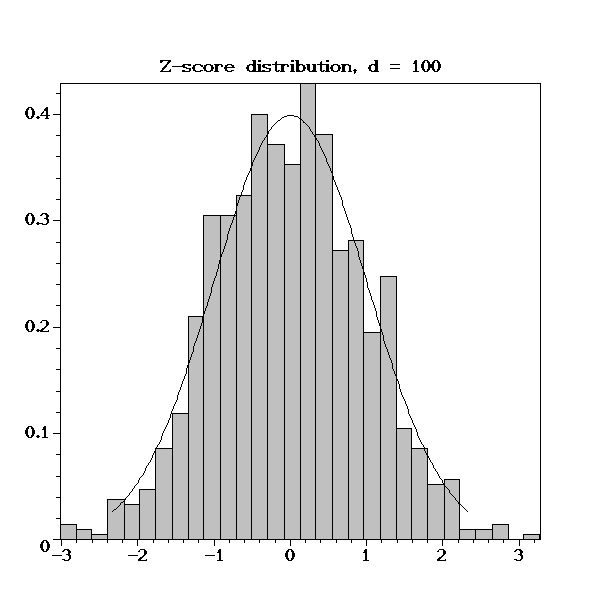
\includegraphics[width=0.5\textwidth]{./z_score_2.jpg} &
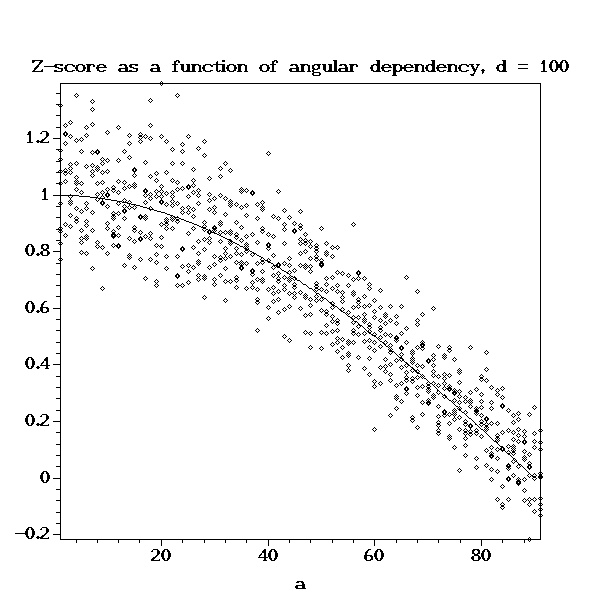
\includegraphics[width=0.5\textwidth]{./z_score_2a.jpg} \\
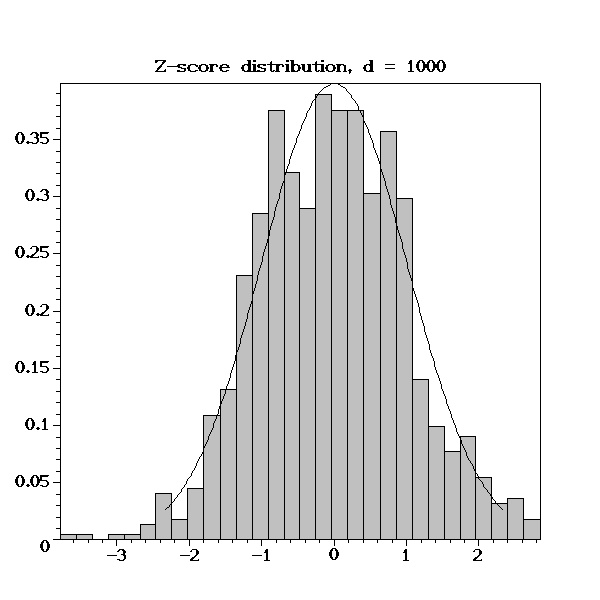
\includegraphics[width=0.5\textwidth]{./z_score_3.jpg} &
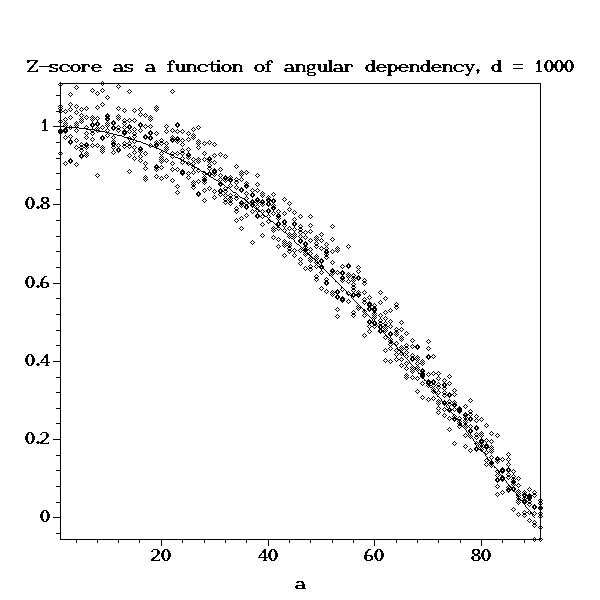
\includegraphics[width=0.5\textwidth]{./z_score_3a.jpg} \\
\end{tabular}}
\caption{Numerical observations of the similarity defined by the dot product of two random vectors for $d=100$ in the upper row and $d=1000$ in the lower row.
  The left column shows the histogram of the z-score ($\sqrt{d} \, ({\bf x} \cdot {\bf y})$) for two normal vectors, in comparison with a normal distribution.
  These experimental distributions have a kurtosis of about $10$; this is lower than the kurtosis of a normal distribution, which is expected to have a kurtosis of $3$.
  The right column shows the z-score as a function of the angle $a \deq \widehat{{\bf x}, {\bf y}} = \mbox{arccos}({\bf x} \cdot {\bf y})$, making it possible to visualize the dispersion with respect to the expected cosine profile.
 }
\label{z_score}
\end{figure}

This makes it possible, on the one hand, to consider, for instance, a $\pm 2$ threshold for the standard deviation, along with considering this z-score to have a confidence interval better than $99\%$, and to relate the similarity estimation to an angular dependence between two vectors, as detailed in Fig.~\ref{z_score}. To the best of our knowledge, this obvious implementation has not yet been made explicit, and it is used in subsection~\ref{macrovsa}, as detailed in Appendix~\ref{algorithmic-ersatz}, allowing us to propose to simulate the different operations defined later in this paper at a macroscopic scale.

\subsection{Modality encoding} \label{modality-encoding}

\subsubsection{The notion of belief}

Most VSA approaches consider that two vectors \textbf{x} and \textbf{y} contain (not exclusively) equivalent information that is semantically equivalent, when the similarity $\tau$ equals 1, but there are different ways to interpret this result. Here, we enrich the notion of something being either false or true using a numeric representation of, e.g., partial knowledge, as illustrated in Fig.~\ref{possibility-necessity}. The true value corresponds to 1 (fully possible and fully necessary), the false value to -1 (neither possible nor necessary, i.e., impossible), and the unknown value to 0, which corresponds to a fully possible but absolutely not necessary value.

\begin{figure}[htbp]
\centerline{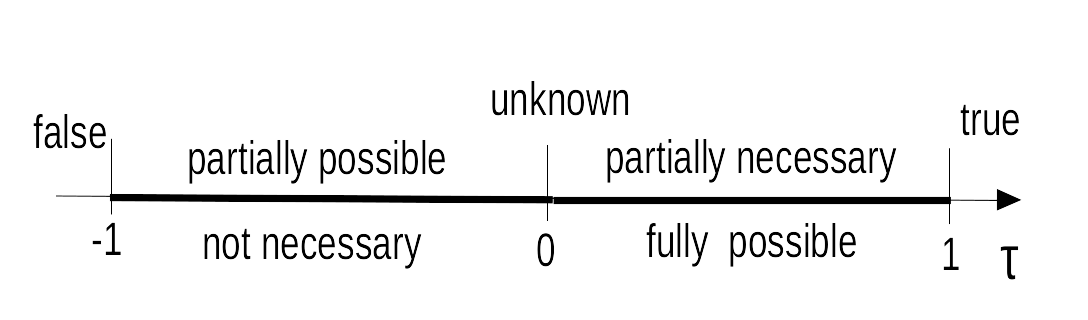
\includegraphics[width=0.8\textwidth]{./possibility-necessity.png}}
\caption{Representation of the partial truth $\tau \in [-1,1]$ with regard to necessity and possibility, as defined in the possibility theory. The interpretation is that what is ``not so false'' is partially possible but not necessary and what is ``partially true'' is entirely possible but partially necessary. Such a formulation corresponds qualitatively to the human appreciation of the degree of belief in a fact.}
\label{possibility-necessity}
\end{figure}

Our representation is in one-to-one correspondence with the dual notions of necessity and possibility representation in the standard possibility theory. Information is always related to a certain degree of what is called ``belief'' in this formalism. While almost all partially known information is related to probability, the human ``level of truth'' is more subtle and related to possibility and necessity, as formalized in the possibility theory discussed in \cite{denoeux_representations_2020} and \cite{denoeux_representations_2020-1}. This theory stems from modal logic, i.e., something being true in a ``given context'' \cite{fischer_modal_2018}, which is also considered representative of what is modeled in educational science and philosophy \cite{rusawuk_possibility_2018}; namely, it corresponds to common-sense reasoning in the sense of Piaget \cite{smith_development_1994}, which involves taking exceptions into account, i.e., considering non-monotonic reasoning. In other words, possibility theory is devoted to the modeling of incomplete information, which is related to an observer's belief regarding a potential event and surprise after the event's occurrence. Furthermore, in symbolic artificial intelligence, i.e., knowledge representation and logical inference, a link has been drawn between this necessity/possibility dual representation and ontology \cite{tettamanzi_possibilistic_2017}. This must be understood as a deterministic theory, in the sense that partial knowledge is not represented by randomness\footnote{This deterministic representation of partial knowledge can be generalized in order to also include a representation of the randomness belief. In the vanilla possibility theory, the possibility can be seen as an upper probability: Any possibility distribution defines a set of admissible probability distributions, i.e., a consonant plausibility measure in the Dempster–Shafer theory of evidence \cite{beynon_dempstershafer_2000}. In \cite{vallaeys_generaliser_2021,vieville_representation_2022}, it is proposed to bound the approximate probability, reconsidering the original notion of necessity, in order to also consider a lower bound of probability. This could be an interesting extension of the present work.}.
This modal notion of partial belief is not only epistemic or doxastic but also deontic and so on, i.e., it has several semantic interpretations, depending on the concept feature.
This representation has also been designed to be compatible with the ternary Kleene logic, in addition to being coherent with respect to the possibility theory, as discussed in detail in \cite{vieville_representation_2022}, where this deterministic representation of partial knowledge is generalized in order to include a probabilistic representation (using a 2D representation). 

\subsubsection{Implementing partial similarity knowledge}

Let us now propose a design choice to apply this quantification to symbols. A symbol representing a piece of information with a partial degree of belief $\tau \in [-1, 1]$ could be defined as:
\eqline{\hat{\mathbf{x}} \defq \tau \, \mathbf{x},}
where $\mathbf{x}$ corresponds to the numerical grounding of a symbol, and $\hat{\mathbf{x}}$ corresponds to the numerical grounding of a symbol, given its degree of belief $\tau$.

Interestingly enough, this representation is coherent with the semantic similarity in the following sense: Are two vectors containing similar information? Considering $\mathbf{x} \cdot \mathbf{y}$, if this value is close to $1$, then it is considered true, and the modal representation and semantic similarity are coherent. If it is almost equal to $0$, then the modal representation is {\em not true}. Since our design choice is to consider being in an open world in which all that is not true is not necessarily false, but that we simply can not claim is its true, say it is unknown. To take this a step further, if this value is negative (down to $-1$), the modal representation considers that it is false, i.e., that the contrary is true, which is coherent with the semantic similarity, although negative values are not explicitly used, to the best of our knowledge, in the literature quoted in this paper.

Given these atomic ingredients, let us now study how they can be used in different cognitive data structures.

\section{Knowledge structure encoding}

\subsection{Knowledge representation}

From early artificial intelligence knowledge representations such as previously avowed frameworks to modern web semantic data structures, the basic idea of symbolic representation is to consider symbols that represent objects and express knowledge through relationships, i.e., triple statements of the form {\tt (\$subject, \$predicate, \$object)}, as schematized in Fig.~\ref{triple}.

\begin{figure}[htbp]
\centerline{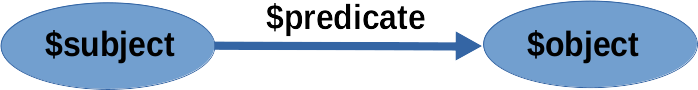
\includegraphics[width=0.5\textwidth]{./triple.png}}
\caption{Atomic representation of knowledge: To express some knowledge regarding a symbol, the subject, we define a feature with a predicate that has an object as an attribute (i.e., a quantitative data value or a qualitative symbol).}
\label{triple}
\end{figure}

Following, e.g., \cite{gardenfors_conceptual_2004}, we start by introducing the notion of a concept, represented by a symbol encoded in a hypervector. Several symbols may be elements of such a concept. A concept corresponding to a unique symbol, i.e., a singleton, corresponds to an individual. Concepts, in, \cite{gardenfors_conceptual_2004} are specified with the simple common idea that a concept can be defined by ``feature dimensions,'' i.e., attributes with some typed value. The object can be either qualitative or quantitative ``data'' or another object that describes relations between objects. This is also the basic syntax of ontology languages. In the brain, such feature dimensions are usually anchored in sensorimotor feature spaces \cite{freksa_strong_2015}, in coherence with the present representation. Furthermore, given a concept, as developed in \cite{gardenfors_conceptual_2004}, this choice of representation induces the notion of prototypes, which makes it possible to represent the state space region corresponding to the concept.

Taking this a step further, the definition of a concept is completed by relations between concepts, i.e., predicates. Predicates can be generic, in the sense of, e.g., \cite{mcclelland_parallel_2003}, defining a hierarchical taxonomy using the ``{\tt is-a}'' predicate, as in almost any such language, but they also have capability qualities (``{\tt can}''), extrinsic qualities (``{\tt has}''), and intrinsic qualities (``{\tt is}''); thus, there are four general predicates. They can also be unconstrained, as in the RDFS framework (see, e.g., \cite{noy_ontology_2001} for an introduction), describing any property, and in that case, properties also form a taxonomy\footnote{For instance, stating that {\tt Amid is-a-descendant-of Yang-Li} implies that {\tt Amid is-a-relative-of Yang-Li}, the former property is a sub-property of the latter. This example also illustrates that such properties have meta-properties, such as being transitive or symmetric.}. This is further illustrated in subsection~\ref{hierarchical}. Conversely, as a limit case, we could consider relationships between subjects and objects only, without taking into account the nature of a relationship (predicate) or its direction.

An important point is that features can be hierarchical because the value itself may have some features: For instance, a quantitative physical value is not just a ``number'' stating the current or default value. It may also be specified by a unit and a precision value or some bounds. In terms of the data structure, this forms a tree, and the whole data structure is a set of trees, i.e., a forest, and thus it is a graph.

We are going to specify how we can represent such symbolic information at a biologically plausible level in the present study using VSAs.

\subsection{Hierarchical schematic organization of information} \label{hierarchical}

To make things more concrete, we aim at manipulating the symbolic representation of knowledge of the form shown in Fig.~\ref{concept-grounding}.

\begin{figure}[htbp]
\centerline{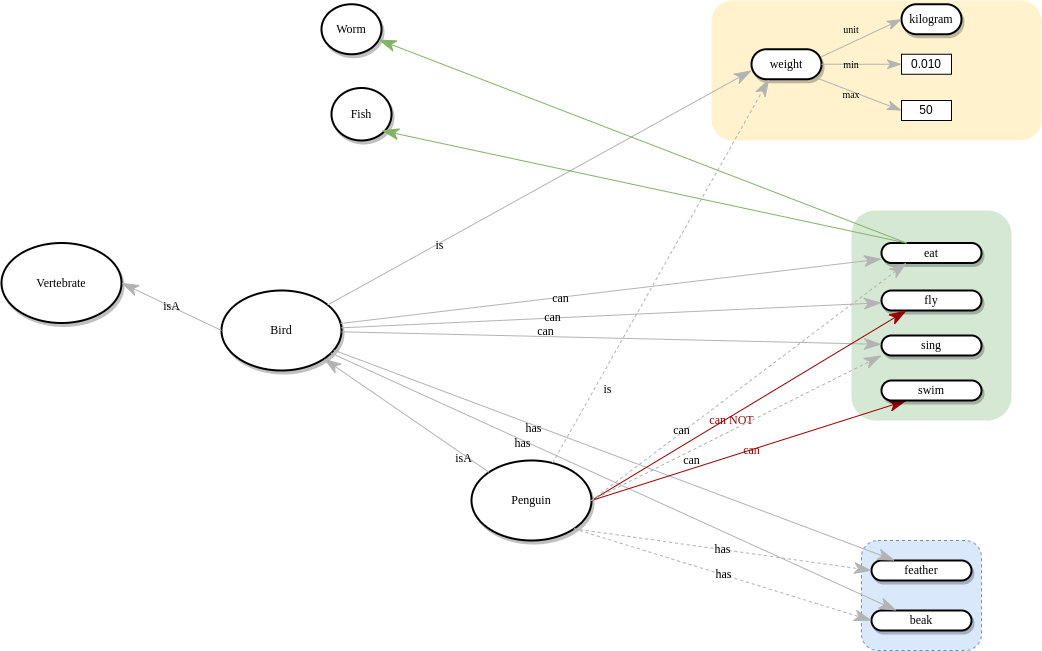
\includegraphics[width=\textwidth]{./concept-grounding.png}}
\caption{In our context, we represent concepts as a hierarchical data structure. Concepts are anchored in an input/output, i.e., stimulus/response, framework, which might consist of sensorimotor feature spaces (colored regions) corresponding, for example, to different sensor modalities. Inherited features (e.g., the penguin “is-a” bird and thus inherits the features of a bird) are shown with dotted lines, while red lines represent overwritten values (e.g., a penguin can also swim but cannot fly). Green arrows point toward concepts that are themselves attributes of other concept features, accounting for inter-concept relationships.
Values are completed by meta-information that is not explicitly manipulated by the agent but is used for process specification or interpretation (e.g., the weight unit and bounds).}\label{concept-grounding}
\end{figure}

In other words, we follow \cite{gardenfors_conceptual_2004}, with the simple idea that an individual resource can be defined by ``feature dimensions,'' i.e., attributes with some typed value. For instance, a bird could be the following\footnote{The syntax used is a weak form of the \href{JSON}{https://www.json.org} syntax: \hhref{https://line.gitlabpages.inria.fr/aide-group/wjson}.}:

\begin{lstlisting}[basicstyle=\small]
bird: {
  is_a: vertebrate
  can: { sing fly eat: { worm fish } }
  has: { feather beak }
  is: { weight : { min: 0.010 max: 50 unit: kilogram } }
},\end{lstlisting}
with some exceptions like penguins:
\begin{lstlisting}[basicstyle=\small]
penguin: {
  is_a: bird
  can: { fly: false walk }
}.
\end{lstlisting}

Equivalently, this could be decomposed\footnote{Conceptually, considering a distributed version of this hierarchical specification by enumerating each node and the directed edge is rather obvious; at the concrete implementation level, some details have to be carefully taken into account and the so-called \href{turtoise}{https://line.gitlabpages.inria.fr/aide-group/wjson/turtoise.pdf} specification takes care of proposing a well-defined one-to-one correspondence (with an open-source implementation). It is not necessary to describe this in detail here.} in terms of triples such as {\tt bird is\_a vertebrate} and so on.

Here, we choose the general approach of semantic knowledge representation using a hierarchical taxonomy ({\tt is-a}) with capability features ({\tt can}), including those related to other resources, extrinsic features ({\tt has}), and intrinsic features ({\tt is}) \cite{mcclelland_parallel_2003}\footnote{Quoting the authors {\em In this approach, the four propositional relations from Quillian’s hierarchy are viewed as distinct contexts. The "is a" relation corresponds to a naming or explicit categorization context, in which the object’s name or category label is of relevance, as these might be indicated verbally (e.g., by a sentence such as “This is a bird” or “This is a canary”). The can relation corresponds to a context in which the behaviors of the object might be observed; the is relation corresponds to a context in which its appearance properties are highlighted; and the has relation corresponds to a context in which its parts are highlighted.}}.
A more granular partition could be envisioned, but this illustrative example is sufficient to allow us to detail the main characteristics of our representation.
Some features are properties, and others are relations. A property can be qualitative, e.g., the {\tt is-covered-by} property takes a value in an enumeration (e.g., \{{\tt sing}, {\tt fly}\}), or quantitative (e.g., the {\tt weight}). The features can be hierarchical, either because the value is an enumeration (e.g., {\tt can}) or because the value has some features (e.g., {\tt weight}). \vthierry{For instance, the statement ``Zheng-You speaks Sundanese'' means ``Zheng-You can [has the capability to] speak Sundanese'', while the statement ``Zheng-You is speaking Sundanese'' describes an ongoing action rather than a concept attribute, while the statement ``Leila likes kiwis'' means ``Leila has kiwis in her favorite fruits set''. These four verbs seem sufficient, as developed by the authors to describe concept properties in the wide sense. Choosing such normalized representation allows us to better represent knowledge in a canonical form.}

Such a data structure defines a ``concept'' in the sense of \cite{gardenfors_conceptual_2004} (e.g., ``a bird''), which is both a convex region of the state space (e.g., the region of all birds) and a prototype: Each feature has a default value, and this also defines a prototype (e.g., a typical, i.e., prototypical, bird). It corresponds to the third cognitive memory architecture, as proposed by \cite{eichenbaum_memory_2017}, and we are now going to discuss how to implement it in a VSA framework.

Let us now review how such a cognitive symbolic data structure can be implemented in a biologically plausible way using the proposed VSA framework. 

\subsection{Biologically plausible implementation} \label{plausible-implementation}

To proceed, we thus have to consider a set of items of knowledge of the form shown in Fig.~\ref{triple} bounded to a triple of vectors $\{(\mathbf{s}_1,  \mathbf{p}_1,  \mathbf{o}_1.), \cdots (\mathbf{s}_N,  \mathbf{p}_N,  \mathbf{o}_N.)\}$. This corresponds to relations, which are the basis of semantic information.

\subsubsection{Using bundling and binding to store information} \label{containers}

As developed in detail in Appendix~\ref{data-structure} and summarized in Table~\ref{containers-table}, the VSA formalism makes it possible to implement different data structures corresponding to different memory architectures, as defined by \cite{eichenbaum_memory_2017}, and to different programming containers. The key point of the present work is, on the one hand, to verify that these VSA mechanisms generalize to modal symbol encoding, which is technically obvious (see Appendix~\ref{data-structure}) but worthwhile to mention, and, on the other hand, to show that they also very easily generalize to the so-called ``relational map,'' as developed in the next subsection. Further details on a scalable biologically plausible knowledge representation can be found in \cite{crawford_biologically_2016}.

\begin{table}[htbp]
  \begin{center}\begin{tabular}{|c|c|c|c|}
      \hline
     \parbox[u]{0.2\textwidth}{Container} & \parbox[u]{0.2\textwidth}{VSA mechanism} & \parbox[u]{0.2\textwidth}{Cognitive usage} & \parbox[u]{0.3\textwidth}{Main available operations} \\
\hline
     \parbox[u]{0.2\textwidth}{Set} & \parbox[u]{0.2\textwidth}{Bundling or superposition} & & \parbox[u]{0.3\textwidth}{~\\+ Element insertion/modification \\ + Check membership \\ - No enumeration\\} \\
\hline     
     \parbox[u]{0.2\textwidth}{Map or dictionary} & \parbox[u]{0.2\textwidth}{Binding superposition} & \parbox[u]{0.2\textwidth}{Associative memory} & \parbox[u]{0.3\textwidth}{~\\+ Element insertion/modification \\ + Value·s retrieval from key\\ + Key·s retrieval from value \\ + Exact symbol recovery from approximate input \\ - No enumeration\\} \\
\hline     
     \parbox[u]{0.2\textwidth}{Indexed and chained list} & \parbox[u]{0.2\textwidth}{Ordinal binding superposition} & \parbox[u]{0.2\textwidth}{Sequential memory} & \parbox[u]{0.3\textwidth}{~\\+ Element insertion/modification \\ + Value enumeration\\} \\
\hline     
     \parbox[u]{0.2\textwidth}{Relational map} & \parbox[u]{0.2\textwidth}{(see next subsection)} & \parbox[u]{0.2\textwidth}{Hierarchical memory} & \parbox[u]{0.3\textwidth}{~\\+ Element insertion/modification \\ - No enumeration\\} \\
\hline     
 \end{tabular} \end{center}~\\
\caption{Biologically plausible data containers; see Appendix~\ref{data-structure} for details.} \label{containers-table}
\end{table}

\subsubsection{Relational maps} \label{relational-map}

How should we such information in a biological data structure? As developed previously all knowledge is decomposed in the form of triples, as shown in Fig.~\ref{triple}, i.e., in the form of relations between entities. We now discuss how to implement such a distributed representation, a kind of ``triple store'' using superposition, i.e., bundling, and a few binding operations, i.e., a {\em relational map}. The most natural choice might be to consider the triple set $\mathcal{T}$ grounded to a vector $\mathbf{t}$:
\eqline{\mathbf{t}_{\mathbf{pso}} \defq \sum_i \mathbf{B}_{\mathbf{p}_i} \, \mathbf{B}_{\mathbf{s}_i} \, \mathbf{o}_i.}
Here,
\\ - $\mathbf{o}_i$ represents vectors encoding symbols;
\\ - quantities of the form $\mathbf{B}_{\mathbf{y}}$ are binding matrices that make it possible to create a $\mathbf{B}_{\mathbf{y}} \, \mathbf{x}$ key-value pair (the key is $\mathbf{y}$ and the value is $\mathbf{x}$), as defined in equation~(\ref{eq-binding}) of Appendix~\ref{VTB-algebra};
\\ - combining these quantities to create a vector $\mathbf{B}_{\mathbf{p}_i} \, \mathbf{B}_{\mathbf{s}_i} \, \mathbf{o}_i$ makes it possible to encode a triple as a new random vector, i.e., as a neuronal ensemble activity; and
\\ - finally, the sum makes it possible to superpose a different triple. A reader not familiar with this VSA formalism will find in Appendix~\ref{data-structure} a didactic introduction, while the choice of the binding operator from among several available binding operators \cite{schlegel_comparison_2020} is discussed in Appendix~\ref{VTB-algebra}. For this section to be self-contained, one just has to consider that binding makes it possible to create a key-value symbol pair, while the unbinding operation, which is written as $\mathbf{B}_{\mathbf{y}^\sim}$, makes it possible to retrieve the value from the key, as discussed below. 

This design corresponds to a nested associative map: Each property $\mathbf{p}_j$ is defined through a mapping between subjects and objects\footnote{
Obviously,
\eqline{B_{\mathbf{p}_j^\sim} \, \mathbf{t}_{\mathbf{pso}} =
  \sum_{i, \mathbf{p}_j \neq \mathbf{p}_i} B_{\mathbf{p}_j^\sim} \, \mathbf{t}_{\mathbf{p}_i} +
  \sum_{i, \mathbf{p}_j = \mathbf{p}_i}  B_{\mathbf{p}_j^\sim} \, \mathbf{B}_{\mathbf{p}_i} \, \mathbf{B}_{\mathbf{s}_i} \, \mathbf{o}_i \simeq \mathbf{t}_{\mathbf{p}_j}.}
The first term vanishes because $\mathbf{t}_{\mathbf{p}_i}, \mathbf{p}_j \neq \mathbf{p}_i$, is generically orthogonal to $\mathbf{p}_j^\sim$, while the second reduces to $\mathbf{t}_{\mathbf{p}_j}$ thanks to the approximate inverse property.}:
\eqline{\mathbf{t}_{\mathbf{p}_j} \defq \sum_{i, \mathbf{p}_j = \mathbf{p}_i} \mathbf{B}_{\mathbf{s}_i} \, \mathbf{o}_i = B_{\mathbf{p}_j^\sim} \, \mathbf{t}_{\mathbf{pso}}.}

Given a triple $(\mathbf{s}_0,  \mathbf{p}_0,  \mathbf{o}_0.)$, it is straightforward to verify to what extent it is stored in the relational map through unbinding:
\eqline{(B_{\mathbf{s}_o^\sim} \, B_{\mathbf{p}_o\sim} \, \mathbf{t}_{\mathbf{pso}} \cdot \mathbf{o}_0),}
and this obviously generalizes to a triple multiplied by a modal $\tau$ value.

We can also further obtain all objects of a given subject for a given property,
\eqline{\mathbf{t}_{\mathbf{p}_j, \mathbf{s}_j} \defq \sum_{\mathbf{p}_j = \mathbf{p}_i, \mathbf{s}_j = \mathbf{s}_i} \mathbf{o}_i \simeq B_{\mathbf{s}_j^\sim \oslash \mathbf{p}_j^\sim} \, \mathbf{t}_{\mathbf{pso}}, }
using the notation of Appendix~\ref{VTB-algebra}. We can also easily define
\eqline{\mathbf{t}_{\mathbf{p}_j, \mathbf{o}_j}  \defq \sum_{\mathbf{p}_j
  = \mathbf{p}_i, \mathbf{o}_j = \mathbf{o}_i} \mathbf{s}_i
  \simeq B_{\mathbf{s}_j^\sim} \, \mathbf{B_{\leftrightarrow}} \, B_{\mathbf{p}_j^\sim} \, \mathbf{t}_{\mathbf{pso}}.}

A dual construction, $\mathbf{t}_{\mathbf{spo}} \defq \sum_i \mathbf{B}_{\mathbf{s}_i} \, \mathbf{B}_{\mathbf{p}_i} \, \mathbf{o}_i$, with similar decoding formulae makes it possible to further access the properties of a given subject $\mathbf{t}_{\mathbf{s}_j} \defq \sum_{i, \mathbf{s}_j = \mathbf{s}_i} \mathbf{B}_{\mathbf{p}_i} \, \mathbf{o}_i$ or the properties of a given subject-object couple $\mathbf{t}_{\mathbf{s}_j, \mathbf{o}_j} \defq \sum_{i, \mathbf{s}_j = \mathbf{s}_i, \mathbf{o}_j = \mathbf{o}_i} \mathbf{p}_i$ using similar formulae. We thu shave now two relation maps $\mathbf{t}_{\mathbf{pso}}$ and $\mathbf{t}_{\mathbf{spo}}$.
A key point is that, to the best of our knowledge, there is no operation to recover $\mathbf{t}_{\mathbf{s}_j}$ or $\mathbf{t}_{\mathbf{s}_j, \mathbf{o}_j}$ from $\mathbf{t}_{\mathbf{pso}}$, and no operation to recover $\mathbf{t}_{\mathbf{p}_j}$ or $\mathbf{t}_{\mathbf{p}_j, \mathbf{o}_j}$ from $\mathbf{t}_{\mathbf{spo}}$. This is an important constraint, and it would be interesting to verify if such a constraint is observed at the level of the brain's semantic memory.

Moreover, in order to enumerate the different elements of these maps $\mathbf{t}_{\bullet}$, we need the corresponding indexing mechanisms discussed previously. If the basic operation is to enumerate all triples, with order constraints, then the choice of the storage architecture is not crucial; this is going to be the case later in this paper.

To take this a step further, we can also consider an additional symbol ``something,'' and each time a triplet $(\mathbf{s}_i,  \mathbf{p}_i,  \mathbf{o}_i.)$ is added, we can also add $(\mathbf{\sigma},  \mathbf{p}_I,  \mathbf{o}_i.)$, $(\mathbf{s}_i,  \mathbf{\sigma},  \mathbf{o}_i.)$, and $(\mathbf{s}_i,  \mathbf{p}_I,  \mathbf{\sigma}.)$. This makes it possible to retrieve the fact that there is a link between the predicate and object, subject and object, and subject and predicate, without requiring the enumeration of the different elements, as previously discussed.

At the cognitive level, this corresponds to cognitive maps interacting with each other and is a proposal to formalize the notion of hierarchical memory organization, as discussed in, e.g., \cite{eichenbaum_memory_2017}.

At the computer programming level, this corresponds to a ``triple store'' used in ontology reasoners and is in fact a distributed representation of an oriented graph, in the form of an adjacency set for $\mathbf{t}_{\mathbf{spo}}$ construction and a hierarchical edge set for $\mathbf{t}_{\mathbf{pso}}$ construction.

At this stage, we have reviewed and developed the VSA elements needed for the next step, in particular the notion of a relational map, which is a combination of associative maps enumerated by an indexed list that builds on the bundling structure reviewed at the beginning of this section. We are now going to explain how symbolic computation can be performed by making such memory structures interact.

\section{Knowledge transformation encoding} \label{transformation}

Let us now consider how to define operators that make it possible to enrich the memorized information using biologically plausible transformations.

\subsection{Considering symbolic operations}

We are going to consider symbolic operations as entailment rules of deductive, inductive, or abductive inference. It is worthwhile to note that both induction, as, for instance, in \cite{domingos_unifying_1996}, and abduction could be formalized by inference rules (see, e.g., \cite{lakkaraju_rule_2000} for a computational example and \cite{shanahan_abductive_2000} for a contribution regarding temporal reasoning). Our position is that reasoning in the brain is mainly related to the construction of mental models, as discussed in, e.g., \cite{khemlani_causal_2014}, considering common-sense reasoning. Such a framework better corresponds to human reasoning than pure logic reasoning, including modal logic reasoning \cite{ragni_reasoning_2018}. In any case, a mechanism to construct, enrich, and modify such a mental model must be described.

Here, we focus on rule-based reasoning. Regarding an ontology such as OWL\footnote{\url{https://en.wikipedia.org/wiki/Web_Ontology_Language}} semantic web knowledge representation language family, the RDF Schema (RDFS)\footnote{\url{https://en.wikipedia.org/wiki/RDF_Schema}} layer (see Appendix~\ref{RDFS-entailment-rules} for a detailed presentation) is purely rule-based, and several property inferences such as the inverse, symmetry, transitivity, and rules of equating objects are rule-based. This corresponds to the so-called OWL 2 RL profile. It allows scalable reasoning without sacrificing too much expressive power and can be implemented using rule-based reasoning mechanisms\footnote{See, for instance, \hhref{https://www.w3.org/TR/owl2-profiles/\#OWL_2_RL} for details.}. By carefully considering the related entailment rules of this specification, we have observed that they require either one, two, or at most three premises, which is an important aspect in our context. Beyond this, other rule-based mechanisms can complete the description of rule-based reasoning, such as by adding function-free Horn rules (e.g., using the SWRL\footnote{\hhref{https://en.wikipedia.org/wiki/Semantic_Web_Rule_Language}} language with suitable conditions \cite{motik_query_2005}). This is what we target here.

Beyond deductive reasoning, following \cite{domingos_unifying_1996}, for instance, or using inductive logic programming\footnote{\hhref{https://en.wikipedia.org/wiki/Inductive_logic_programming}}, inductive reasoning is easily formulated using the rule-based mechanism provided; we can add counting operations in order to perform enumerative induction. This means that we will have rules that are going to scan the whole relational map, but we are going to observe that this is also required for other rules. This being stated, we will not further develop this aspect, and it is only mentioned as an interesting perspective of the present work.

Taking this a step further, rule-based abduction has been formalized, following, e.g., \cite{lakkaraju_rule_2000}, as in fact a set of possible causes of a given observation that is deduced (to make short a more sophisticated story). In this rather restricted but still powerful context, the rule-based mechanism does not ``invent'' the cause but does infer parameterized predefined causes, performing what could be called model-based abduction.

To summarize, our design choice is to propose a rather generic mechanism, specific enough to produce a robust implementation and make it possible to specify what has been reviewed here.

\subsection{A generic mechanism}

In order to proceed, let us write
\eqline{(\mathbf{\$s}_0,  \tau_0 \, \mathbf{\$p}_0,  \mathbf{\$o}_0 .),}
which represents the fact that a variable subject $\mathbf{\$s}_0$ is associated with a variable object $\mathbf{\$o}_0$ in an associative table related to the predicate variable $\mathbf{\$p}_0$ with a level of belief $\tau_0$, i.e., in the triple store,
\eqline{\mathbf{t}_{pso} = \tau_0 \, \mathbf{B}_{\mathbf{\$p}_0} \, \mathbf{B}_{\mathbf{\$s}_0} \, \mathbf{\$o}_0 + \cdots,}
where we use the $\$$ prefix to make explicit the fact that a given symbol is a variable symbol.

We are going to consider entailment rules of the form
\eqline{\bigwedge_{i=1}^{i=I} (\mathbf{\$s}_i,  \mathbf{\$p}_i,  \mathbf{\$o}_i .) \rightarrow \bigoplus_{j=1}^{j=J} (\mathbf{\$s}_j,  \tau_j(\cdot) \, \mathbf{\$p}_j,  \mathbf{\$o}_j .),}
where
\begin{itemize}
\item The left-hand-side expression corresponds to a conjunction of premises, with $\mathbf{\$x}_i$ ($\mathbf{\$x}$ stands for the subject, predicate, or object) receiving the corresponding item as input.
\item The weight $\tau_j(\cdot)$ is a function of left-hand-side elements; it is equal to $0$ if the rule does not apply to the element, it is negative if the consequence is to partially delete an element, and it is positive otherwise.
\item Each right-hand-side value $\mathbf{\$x}_j$ ($\mathbf{\$x}$ stands for the subject, predicate, or object) is either a constant or equals a left-hand-side element $\mathbf{\$x}_i$, or it could be a more complex expression of left-hand-side elements.
\item The right-hand-side expression corresponds to $\mathbf{t}_{pso} \mathrel{+}= \sum_j \tau_j(\cdot) \, \mathbf{B}_{\mathbf{\$p}_j} \, \mathbf{B}_{\mathbf{\$s}_j} \, \mathbf{\$o}_0$, i.e., it updates the related structure. In almost all the cases that we have considered, only one triple is generated; this part of the setup is thus stated for future use.
\end{itemize}

This includes modifying (including deleting) existing triplets since they are weighted by a $\tau$ value that can be modified and thus set to $0$. The key point is that the calculation of $\tau_j(\cdot)$ allows the integration of not only modal logical formulae but also threshold mechanisms or counting operations that are required for induction.

Such a general setting clearly corresponds to the usual production rules. In the binary mode, e.g., if $\tau \in \{0, 1\}$, this is nothing but a specification equivalent to Horn clauses. Introducing the calculation of $\tau_j(\cdot)$ allows us to go beyond this, but at the cost of lowering the decidability and implementation tractability, as detailed later in this paper, so we will need to consider suitable convergence conditions.

At the implementation level, the application of such rules can simply be implemented using feedback connections between an iterator over the triples of the relational map, as discussed in detail for a typical example before a general implementation is described.

\subsection{Class inheritance entailment rule} \label{inheritance}

In order to better understand what is proposed here, let us start by detailing an illustrative and quite universal example.

\subsubsection{Class inheritance as a major deductive mechanism}

The most common entailment rule is likely the class inheritance rule, which states that ``if a subject belongs to a class, and if this class is a subset of a superclass, then the subject belongs to the superclass,'' e.g., ``if Tom is a cat, and cats are animals, then Tom is an animal.'' This is a deductive rule, i.e., a particular syllogism, which belongs to common-sense reasoning and is well understood as soon as formal reasoning emerges in children \cite{smith_development_1994}.

The notion of ``class'' corresponds to Boolean properties (e.g., if you are alive, you belong to the class of living organisms) and capabilities (e.g., if you can fly, you belong to the class of flying organisms). It is associated with a given individual feature. In addition, such Boolean features are organized in a hierarchy, leading to a taxonomy that describes the information about the considered individuals.

At the syntax level, it is based on two predicates, namely, $\texttt{\bf is\_a}$, which states that an individual belongs to a class, and $\texttt{\bf are}$, which states that all individuals of a class are also individuals of a more general class. They correspond, respectively, to $\texttt{\bf rdf:type}$ and $\texttt{\bf rdfs:subClassOf}$ when the RDFS vocabulary is used, as discussed in Appendix~\ref{RDFS-entailment-rules}.

The implementation of the class inheritance rule using the VSA has already been successfully developed and numerically tested in \cite{mercier_ontology_2021} using the Nengo simulator \cite{bekolay_nengo_2014}, while we propose here to rely on this work to propose a more general mechanism. In Appendix~\ref{RDFS-entailment-rules}, we make explicit the fact that the mechanisms of a commonly used semantic web modeling language, the Resource Description Framework Schema (RFDS), can be implemented in such a numerical framework.

\subsubsection{Design of the inference rule}

The class inheritance rule can be written in its ``binary equality'' form as follows:
\eqline{(\mathbf{\$s} ,  \texttt{\bf is\_a} ,  \mathbf{\$c}_1 .) \wedge (\mathbf{\$c}_1 ,  \texttt{\bf are} ,  \mathbf{\$c}_2 .) \Rightarrow (\mathbf{\$s} ,  \texttt{\bf is\_a} ,  \mathbf{\$c}_2 .),}
which states that if any subject $\$s$ belongs to the class $\mathbf{\$c}_1$, i.e., is of ``type'' $\mathbf{\$c}_1$, and this class $\mathbf{\$c}_1$ is a subclass of $\mathbf{\$c}_2$, then $\mathbf{\$s}$ also belongs to the class $\mathbf{\$c}_2$. Here, the equality is either verified or not; we are in the exact reasoning case.

When considering an approximate form, as schematized in Fig.~\ref{rdfs9-derivation}, the rule is written as follows:
\eqline{(\mathbf{\$s}_1 ,  \mathbf{\$p}_1 ,  \mathbf{\$o}_1 .) \wedge (\mathbf{\$s}_2 ,  \mathbf{\$p}_2 ,  \mathbf{\$o}_2 .) \Rightarrow (\mathbf{\$s}_1, \tau \, \texttt{\bf is\_a}, \mathbf{\$o}_2 .),}
with
\eqline{\tau \defq (\mathbf{\$p}_1 \cdot \texttt{\bf is\_a}) \And (\mathbf{\$o}_1 \cdot \mathbf{\$s}_2) \And (\mathbf{\$p}_2 \cdot \texttt{\bf are}),}
so that $\tau$ equals $0$ unless the three equalities are at least partially verified. If $\tau$ equals $0$ nothing is inferred, whereas if it is greater than $0$, a new triple is output. It is a forward schema in the sense that given some input data, a new result is inferred. This second form allows approximate correspondences, e.g., $\mathbf{\$p}_1$ can be approximately $\texttt{\bf is\_a}$.

\begin{figure}[htbp]
\centerline{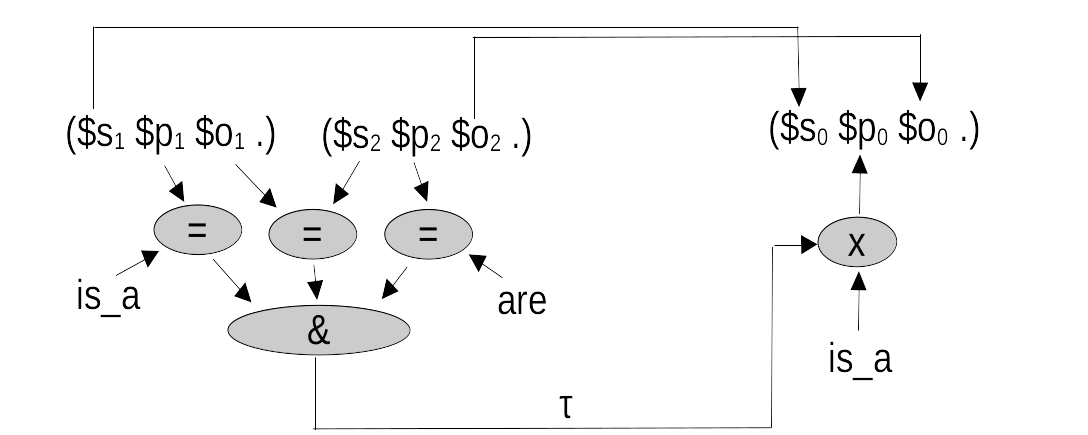
\includegraphics[width=0.75\textwidth]{./rdfs9-derivation.png}}
\caption{The forward implementation of the class inheritance entailment rule.}
\label{rdfs9-derivation}
\end{figure}

The rule requires two numerical operators:
\\- the similarity operator $(\mathbf{x} \cdot \mathbf{y})$, and
\\ - a numerical implementation of the conjunction $(\mathbf{x} \And \cdots \And \mathbf{y})$ operator, which is equal to
\\ \tab \tab - $0$ if one operand is equal to or less than $0$, 
\\ \tab \tab - $1$ if all operands are equal to $1$,
\\ with intermediate values if the operands are between $0$ and $1$.
This could be a $\min$ operator in accordance with the numeric modal logic implementation, as discussed in \cite{vieville_representation_2022}, and this is what we propose here; it is easily implementable\footnote{To be very precise, the $\max$ operator biological implementation is often discussed; it is obviously equivalent to a $\max$ up to linear transform
\eqline{\min(x_1, \cdots x_n) = 1 - \max(1 - x_1, \cdots 1 - x_n), \mbox{ with } x_i \in [0, 1].}} at a neuronal level \cite{bugmann_biologically_1997}, while any other T-norm\footnote{\url{https://en.wikipedia.org/wiki/T-norm}} would be suitable.

\subsubsection{Forward versus backward inference}

This previous setup corresponds to a forward application of the rule, i.e., given two left-hand-side triples, it describes how to numerically calculate the right-hand side.

In its backward form, given the right-hand side, we calculate
\eqline{\begin{array}{rcl}\tau &\defq&  (\mathbf{\$s}_0 \cdot \mathbf{\$s}_1) \And (\mathbf{\$o}_0 \cdot \mathbf{\$o}_2) \And (\mathbf{\$p}_0 \cdot \texttt{\bf is\_a}) \\&& \And (\mathbf{\$p}_1 \cdot \texttt{\bf is\_a}) \And (\mathbf{\$o}_1 \cdot \mathbf{\$s}_2) \And (\mathbf{\$p}_2 \cdot \texttt{\bf are}),\end{array}}
i.e., given a right-hand-side input, we evaluate to what extent two left-hand-side triples could correspond to what is expected. See, e.g., \cite{kapoor_comparative_2016} for an overview of this forward versus backward duality.

In the brain, as discussed, for instance, in \cite{oreilly_goal-driven_2014} at a computational level and \cite{friston_learning_2003} at a more conceptual level, both forward and backward mechanisms are mixed in cognitive behaviors, as studied, for instance, in \cite{amidu_protocol_2019} at a more experimental level. In a nutshell, entailment rules are applied both ``on query'' when, given a goal-directed behavior, some information is required and at a more data-driven level, which here is the stimulus-driven level. In this paper, we are going to focus on forward inference, while in \cite{mercier_ontology_2021}, a backward mechanism based on the VSA, for a specific couple of inference rules, was proposed and validated.

\subsubsection{Exact versus approximate inference}

This rule thus considers approximate similarity: If the input triple states that $\textbf{\$s}_1$ is of class $\textbf{\$o}_1$ only approximately, with $\textbf{\$p}_1 = \tau \, \texttt{\bf is\_a}$, where $\tau \in [0,1]$, and similar approximate equalities, while the similarity operator outputs a value between 0 and 1 and the conjunction operators interpolate values between $0$ and $1$ given the input, we will obtain as the output an appropriate predicate value $\tau' \, \texttt{\bf is\_a}$, with $\tau' \in [0,1]$, which corresponds to the fact that the predicate is only approximately true.

It is interesting to note that in the case of exact inference (i.e., $\textbf{\$p}_1 = \texttt{\bf is\_a}$, $\textbf{\$o}_1 = \textbf{\$s}2$, $\textbf{\$p}_2 = \texttt{\bf are}$), we obtain $\tau = 1$ as expected.

\subsubsection{Implementation of negative inference}

This, however, does not immediately generalize to negative inference (i.e., the fact that it approximately does {\em not} belong to a given class, which is beyond the RDFS specification but present at the OWL level). In this case, a symmetric rule
\eqline{(\mathbf{\$s} ,  \neg \texttt{\bf is\_a} ,  \mathbf{\$c}_1 .) \wedge (\mathbf{\$c}_2 ,  \texttt{\bf are} ,  \mathbf{\$c}_2 .)  \Rightarrow (\mathbf{\$s} ,  \neg \texttt{\bf is\_a} ,  \mathbf{\$c}_2 .)}
has to be considered, with a similar development. The key point is that we must only consider the positive part of the similarity, i.e., it is combined with a rectification operator.

\subsubsection{Implementation of the inference rule}

At the implementation level, what is schematized in Fig.~\ref{rdfs9-derivation} is a simple analog calculation of a $\tau$ value given some left-hand-side input, while the backward implementation is a calculation that also involves the right-hand-side values: It is no more than a weighted connection between triples, i.e., between memory elements, with the generation of a new triple in the forward case and an evaluation of the queried triple in the backward case.

Since we consider approximate inference, and contrary to the binary equality case\footnote{\label{closure} In the binary equality case, let us illustrate our purpose by explicitizing how to generate the entailment rule closure, i.e., all deducible triples, given this rule and a set of input triples. An efficient mechanism must be able to select the pertinent triples, i.e., use a $\textbf{select}$ operator, e.g., based on associative tables, indexed by property and subject. Given two constant values $c_i$ and $c_j$,
\begin{algorithmic}
\ForAll{$(\$s_i \; \$p_i \; \$o_i .), \$p_i = c_i \And \$s_i = c_j$}
\State ../..
\EndFor
\end{algorithmic}
can be enumerated directly without scanning all triples by scanning only the one to be selected. This will allow us to incrementally calculate the closure, given a ``closed'' set of triples $\{(\$s_i \; \$p_i \; \$o_i .) \cdots \}$ with all possible triplets generated and a new triple $(\$s_0 \; \$p_0 \; \$o_0 .)$ to be added. The standard algorithm is written as follows (see, e.g., \cite{kapoor_comparative_2016} for an introduction):
\begin{algorithmic}
\State \textbf{input} A new triple $(\$s_0 \; \$p_0 \; \$o_0 .)$ and a closed set of triples $\{(\$s_i \; \$p_i \; \$o_i .) \cdots \}$.
\State \textbf{let} $\{(\$s_0 \; \$p_0 \; \$o_0 .)\}$ be an ``open'' triple set, initialized with the new triple inside.
\Repeat
\State \textbf{pull} a triple $(\$s_0 \; \$p_0 \; \$o_0 .)$ from the open triple set.
\If{$\$p_0 = \texttt{is\_a}$}
\ForAll{$(\$s_i \; \$p_i \; \$o_i .), \$p_i = \texttt{are} \And \$s_i = \$o_0,$ in the closed triple set}
\State \textbf{add} $(\$s_0 \; \texttt{is\_a} \; \$o_i .)$ to the open triple set.
\EndFor
\ElsIf{$\$p_0 = \texttt{are}$}
\ForAll{$(\$s_i \; \$p_i \; \$o_i .), \$p_i = \texttt{is\_a} \And \$o_i = \$s_0,$ in the closed triple set}
\State \textbf{add} $(\$s_i \; \texttt{is\_a} \; \$o_0 .)$ to the open triple set.
\EndFor
\EndIf
\State \textbf{add} the triple $(\$s_0 \; \$p_0 \; \$o_0 .)$ to the closed triple set.
\Until{the open triple set is empty.}
\end{algorithmic}}, we cannot select triples that exactly match a given pattern. In the forward mode, we must iteratively calculate $\tau(\cdot)$ on the whole conjunction of left-hand-side triples, generating new triples when $\tau(\cdot)$ is above a given threshold, as discussed in the general case below.

\subsection{Entailment rules in the general case}

Going back to the general case, let us now describe an iterative closure algorithm, as schematized in Fig. \ref{tau-architecture}, and discuss its properties.

The key idea is that the relational map is a two-level hierarchy with
\\- a known triples map storing all existing facts and all their derivations given a fixed set of entailment rules, and
\\- a new triples buffer that is input or feedback for entailment rules and for which derivations must still be done.

This is a very common setup used to calculate a fixed point or a closure.

For each new triple, we have to
\\ - check if it is already a known triple; in this case, the job is done;
\\ - otherwise,
\\ \tab - for each entailment rule,
\\ \tab \tab - for each left-hand-side premise instantiated by the new triple,
\\ \tab \tab \tab - for each known triplet set matching the other premises,
\\ \tab \tab \tab \tab - we have to calculate the related $\tau(\cdot)$ value and generate the corresponding new triple or triples; and
\\ \tab \tab \tab \tab - move this new triple from the new triple buffer to the known fact map.

At the initialization stage, the known triple map is empty, and the new triple buffer waits for an input.

\begin{figure}[htbp]
\centerline{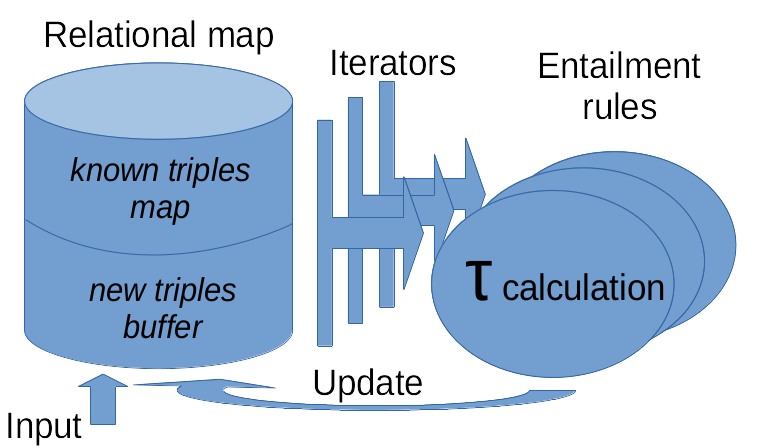
\includegraphics[width=0.8\textwidth]{./tau-architecture.png}}
\caption{The entailment rules feedback mechanism in the general case; see the text for details.}
\label{tau-architecture}
\end{figure}

This basic mechanism raises several issues.

\subsubsection{Comparing a new triple with a known existing triple}

Given the relation map data structure, it is obvious that unbinding can be used to verify if the new triple has a similarity with a known triple of the relation map, as made explicit in subsection~\ref{relational-map}. This similarity corresponds to the product of the degree of belief of each triple and the cosine similarity.

Thanks to the development of a statistical test in section~\ref{encoding} and the easy first-order estimation of the noise level, which is made explicit in Appendix~\ref{algorithmic-ersatz} at the implementation level, we have available, given a probability threshold, a mechanism to decide if the statistical difference between the degrees of belief of the new and known triples is negligible or not.

If it is not negligible, this means that both triples are similar and
\\- either the new triple enforces the degree of belief of the known one, up to the upper bound, which is $1$, corresponding to the ``true'' value,
\\- or it decreases, potentially to the point that it contradicts the previous degree of belief (setting the value to $-1$, which corresponds to the ``false'' value, or setting it to $0$, which corresponds to an ``unknown'' state).

This is very interesting but it has a drawback: It may generate an unstable state. In the binary case, the only degree of belief value is 1, and thus the only possibility is that the new triple equals the known one, meaning that we can avoid redoing the inference. At a more general level, if the only possibility is that the new triple enforces the degree of belief of the known one, we still have to redo inferences, but the system is monotonic, in the sense that the value can only increase and is bounded, and thus the values must converge. A simple way to implement a monotonic mechanism is to take into account the new triple only if its level of belief value is higher than the previously known triple's belief value.

At this stage, it is really a semantic alternative, to be chosen at the application level, depending on whether we design a cumulative knowledge mechanism in a stable universe or an adaptive mechanism in a changing knowledge environment. Both are possible at this implementation level while developing this point is beyond the scope of our purpose.

\subsubsection{Algorithmic complexity for a given new triple}

For one step, given $T$ inputs, $R$ entailment rules of arity $I$ (i.e., number of left-hand-side premises), and $S$ known facts, these nested loops generate $O(T\,R\,I\,S^{I-1})$ calculations of $\tau(\cdot)$. Fortunately, for most of the rules, we have $I=2$ or even $I=1$, except for some fragments of OWL-RL entailment rules\footnote{The situation is even more complex because some entailment rules require the management of a variable arity depending, for instance, on the data structure length. See \cite{cao_web_2014} for a detailed discussion. What we proposed here is thus directly applicable to the RDFS language layer and opportunistically to some OWL 2 reasoning mechanisms.}, which often have $I=3$, so that the complexity is mainly linear with respect to the relational map and seldom quadratic. Furthermore, beyond a sequential system, in our case, we have a completely distributed setup, so that such an operation set is simple to implement in parallel at a certain stage:
\\- Each new triple must be treated in sequence in order to work with a stable known triples map;
\\- however, given a new triple, the rule enumeration, the left-hand-side assignation, and the known triple enumeration on other premises' locations can all be performed in parallel, generating new triples in any order.

\subsubsection{Global algorithmic time and space complexity size}

The global algorithmic complexities in time and space are linked, since each step generates one new triple, while these operations are easily implemented in a distributed framework.

This complexity is highly dependent on each rule; for instance, it is easy to verify that a reflexivity property generates a closure whose order of magnitude is linear with respect to the input triple, a symmetry property generates a closure whose order of magnitude is quadratic with respect to the input triple, and transitivity generates a closure equivalent to the number of paths in an oriented graph, meaning that the complexity can be exponential for a fully connected graph.

Regarding the space complexity, an important aspect is ``catastrophic forgetting,'' i.e., what happens if too many random vectors are superposed in the relation map, meaning that approximate orthogonality cannot be guaranteed. This has been numerically studied in, e.g., \cite{schlegel_comparison_2020}, showing on the one hand that the VT mechanism we have chosen outperforms other representations based on the approximate inverse, and it outperforms other dense methods (but not the sparse one) in terms of the superposition capability. The order of magnitude is rather low, with about 30 symbols reaching 99\% accuracy in a space of dimension 1000, while the best sparse methods have limited performances of about 50 symbols for the same dimension.

As is, the proposed mechanism is limited to toy applications; we have two tracks to improve. On the one hand, when randomly drawing almost orthogonal symbols, it is always possible to use, for instance, the modified Gram-Schmidt methods to improve the stability and obtain precise orthogonality, with the benefit of improving the overall stability. On $N$ symbols, the complexity is quadratic in the number of symbols, i.e., it is $O(d\, N^2)$. On a sphere of dimension $d$, we can obviously draw $d$ orthogonal symbols.

On the other hand, at the microscopic level, in a real spiking neuronal network, the dimension is several orders higher; a neuronal map typically corresponds to a state space of dimension $10^5$, which is not an order of magnitude higher.  Extrapolating the linear approximation of \cite{schlegel_comparison_2020}, which is shown in Fig. 4 of that paper, we obtain a bit more than $3000$ symbols for $d=10^5$ and a bit more than $30000$ symbols for $d=10^6$. 

This is of course impossible to calculate on a mesoscopic scale by manipulating symbols of such a dimension, but we are going to introduce the idea of simulating the VSA mechanism at a macroscopic level, i.e., directly manipulating the algebraic symbols and predicting the cumulative noise of the result. We make explicit this alternative method in Appendix~\ref{algorithmic-ersatz} and share a preliminary implementation of such a mechanism that is no longer limited by the vector space dimension. 

\section{A preliminary experiment}

To illustrate the use of this mechanism, we reconsider the example proposed in \cite{mercier_ontology_2021} and show a minimal ontology in Fig.~\ref{Pizza}, limiting this preliminary experiment to deductive rules and using the RDFs vocabulary. This allows us to better compare the two approaches. Here, the class inheritance \textit{rdfs9} rules described in this paper and the subject domain inference (\textit{rdfs2}), object range inference (\textit{rdfs3}), and property inheritance (\textit{rdfs7}) entailment rules detailed in Appendix~\ref{RDFS-entailment-rules} are implemented (refer to this appendix for an explanation of why this choice makes sense).

\begin{figure}[htbp]
\centerline{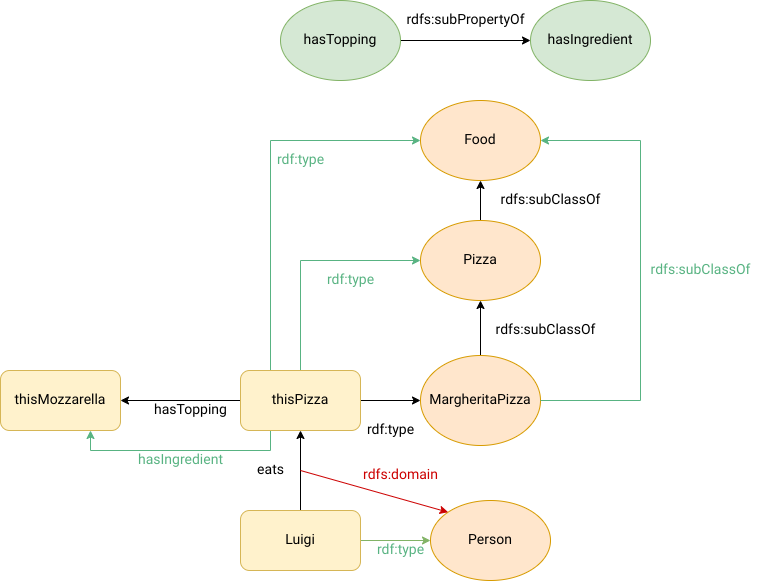
\includegraphics[width=0.8\textwidth]{./pizza-aristotle.png}}
\caption{An example of a simple ontology with three individuals. The black arrows correspond to factual statements input into the database and the green arrows correspond to inferred statements. Rectangular boxes stand for individuals, round boxes stand for classes, and properties are used to label arrows. Here, from the fact that a subject eats an object, we deduce that this subject is a Person, and the object is Food. This is illustrated by a red arrow. From the fact that the object is a Margherita pizza, which is a Pizza, which is a Food, according to the class hierarchy, we deduce that the object is a Pizza, and re-deduce that it is a Food. Furthermore, because Luigi (among other activities, since it is an open world) eats a pizza, we deduce that Luigi is a Person. Because of property heritage, meaning that here a Topping is an Ingredient, we also deduce from the fact that this pizza has mozzarella as a topping that it also has mozzarella as an ingredient. In the macroscopic implementation, this property is deduced from the fact that Margherita pizza always has mozzarella as a topping, allowing us to generate compounded inferences.}
\label{Pizza}
\end{figure}

\subsection{Macroscopic implementation of the VSA system}\label{macrovsa}

As discussed throughout this paper, we are in a position to propose an algorithmic ersatz of the usual VSA mesoscopic linear algebra calculations involving high-dimensional random vectors, and this has been implemented and made available as public documented open-source code\footnote{\hhref{https://line.gitlabpages.inria.fr/aide-group/macrovsa/index.html}}.

For the generation of a symbol, at a given level of belief $\tau$ and for a given level of first-order random normal noise with a standard deviation $\sigma$, the usual similarity, bundling, and binding operations are made available, with some technical details about the noise calculation and software architecture given in Appendix~\ref{algorithmic-ersatz}. We have considered a symbol encoding dimension of $d=256$ to be consistent with previous mesoscopic experiments, such as those in \cite{mercier_ontology_2021}. This is tested with an associative map and relational map, as described in the previous section, and we have implemented the tiny Pizza experiment\footnote{The source code is available at \\ \hhref{https://gitlab.inria.fr/line/aide-group/macrovsa/-/blob/master/src/pizza_experiments.cpp} \\ and it is noticeable that the C/C++ implementation of such rules is straightforward to write, as documented in the source code. This piece of code output is available at \\ \hhref{https://gitlab.inria.fr/line/aide-group/macrovsa/-/raw/master/src/pizza_experiments.out.txt}, \\ in accordance with Fig.~\ref{result0}, and it also shows the intermediate inference steps.}, obtaining, in the simplest case, the expected closure, as given in Fig.~\ref{result0}.

\begin{figure}[htbp]
\begin{center}\begin{tabular}{| p{0.60\linewidth} | p{0.35\linewidth} |}
    {\em Input triples}                            & {\em Inferred triples} \\
\hline
  {\small\tt (Luigi eats thisPizza)}                      & {\small\tt (Luigi rdf:type Person)} \\
  {\small\tt (thisPizza rdf:type MargheritaPizza)}        & {\small\tt (thisPizza rdf:type Pizza)} \\
  {\small\tt (MargheritaPizza rdfs:subClassOf Pizza)}      & {\small\tt (thisPizza rdf:type Food)} \\
  {\small\tt (Pizza rdfs:subClassOf Food)}                & {\small\tt (MargheritaPizza rdfs:subClassOf Food)} \\
  {\small\tt (eats rdfs:domain Person)}                   &  {\small\tt (thisPizza hasIngredient thisMozzarella)}\\
  {\small\tt (eats rdfs:range Food)}                      &\\
  {\small\tt (thisPizza hasTopping thisMozzarella)}       &\\
  {\small\tt (hasTopping rdfs:subPropertyOf hasIngredient)} &\\
  \hline \end{tabular}\end{center}
\caption{The expected inferences using the proposed RDFS subset of entailment rules obtained by
  the macroscopic algorithmic ersatz of the VSA implementation.}
\label{result0}
\end{figure}

More interesting is what happens when modality is considered, e.g.,
\\\centerline{(Luigi 0.5 eats thisPizza).}\\
In other words, it is possible but not completely necessary that Luigi eats the given pizza. In that case,
\\- it is still possible but no longer entirely true that Luigi is a person;
\\- it is still entirely true that this pizza is some food, even if Luigi did not eat it, because it is true that it is a pizza, which is food.
\\ This is what is obtained by the implementation, as shown by the open-source tiny experiment output.

Another interesting aspect is the calculation of the standard deviation of the level of noise modeling that happens at the mesoscopic level for either the calculation of the similarity between two random vectors or unbinding operations. On the one hand, our macroscopic model is consistent with that of \cite{schlegel_comparison_2020}, which obtains the following (from Fig. 4 of that paper) for the VTB representation:
\eqline{d \gtrapprox 32 \, (s + 0.575)}
represents the minimal dimension $d$ needed to obtain a 99\% accuracy with a bundling of size $s$, using a similarity calculation to extract vectors from the bundling. Our model does not take the negligible bias $0.575$ into account but allows us to calibrate the level of noise to $\sigma \simeq \frac{0.016}{d}$, in order to perform a simple z-score test under the normal hypothesis
\eqline{\tau > 2 \, \sigma}
to decide if the related $\tau$ value of the similarity is distinguishable from the noise. On the other hand, we do not consider two vectors to be similar if the similarity is below the standard deviation of the noise, preferring a more conservative threshold.

To take this a step further, we also implemented the $(1/d^{1/4})$ noise dependency for unbinding, with the same calibration, and it would be interesting to further investigate, at the mesoscopic level, the numerical precision of unbinding on associative maps; to the best of our knowledge, this was not studied in the papers quoted here.

Although it is far from being complete, this macroscopic implementation of an algorithmic ersatz of VSA mesoscopic operations seems sound and it is consistent with previous results. It has a final non-negligible advantage: It is quite ``simple'' in the sense that it does not require very complicated or twisted mechanisms. It requires a bit more than 500 lines of formatted C++ code, including formal symbolic operations on the algebraic operators.

\subsection{Comparison with a mesoscopic implementation}\label{nengo}

Let us now discuss how, considering the NEF methodology \cite{eliasmith_how_2013}, as implemented in the Nengo platform \cite{bekolay_nengo_2014}, the previous mechanisms can be implemented at the mesoscopic level. Such an implementation has already been proposed in \cite{mercier_ontology_2021} for the class inheritance \textit{rdfs9} rules detailed in this paper, as a question-answering system, and thus it works in backward mode. In order to avoid lengthening the present paper, we do not describe again all the implementation mechanisms and expected results, but simply explicitize how to implement these mechanisms for this new approach. %Je sais pas si ça va passer mais je trouve ça délicieusement hypocrite … % en effet ^^"

The present implementation works in forward mode, computing the fixed point of the inference loops. To this end, it is possible to create a Nengo vocabulary containing all the resources of our ontology encoded as vectors, and we stored asserted memberships and relationships between these resources in associative memories\footnote{\url{https://www.nengo.ai/nengo-spa/examples/associative-memory.html}}, one for each predicate. For the sake of simplicity, we consider a simplified setup with $\tau = 1$ for each triple, while the use of approximate inference is also discussed in \cite{mercier_ontology_2021} for a Nengo implementation using the VTB operator\footnote{Its transpose (TVTB) can also be used to manage left and right binding: \url{https://www.nengo.ai/nengo-spa/modules/nengo_spa.algebras.html\#nengo_spa.algebras.tvtb_algebra.TvtbAlgebra}.}.

The RDFS entailment rules are implemented as feedback computations, with retro-actions enriching the associative memory's contents, as schematized in Fig.~\ref{architecture_aristotle}. We illustrate here the network connections for \textit{rdfs9} entailments (in forward mode), but similar networks can be implemented for the other rules: 
\\- Two input cues are fed into the network (in this case, they are initialized as TYPE and SUB\_CLASS\_OF because these are the predicates involved in applying the rule). 
\\- Then, each associative memory stores a chained list of all known triples for a given predicate. A feedback connection makes it possible to use the last retrieved value as the key for the next value, making it possible to enumerate the triples just like a relational map, as discussed previously. Retrieved triples are successively stored in a state\footnote{\url{https://www.nengo.ai/nengo-spa/modules/nengo_spa.modules.html?highlight=state\#nengo_spa.modules.State}} that makes it possible to pass data, in this case, to enumerate each input triple, and thus it acts as the input triple buffer of Fig.~\ref{tau-architecture}.
\\ - An action selection module\footnote{\url{https://www.nengo.ai/nengo-spa/modules/nengo_spa.html?highlight=actionselection\#nengo_spa.ActionSelection}} (corresponding roughly to a conditional test) makes it possible to nest the enumeration of the second associative memory by detecting the end of the enumeration of the first associative memory.
\\ - Then, the rule itself is implemented by an interconnection similar to the one made explicit in Fig.~\ref{rdfs9-derivation}, and another selection module acting as a threshold gate triggers the addition of a new triple if the rule is applicable.


\begin{sidewaysfigure}[htbp]
\centerline{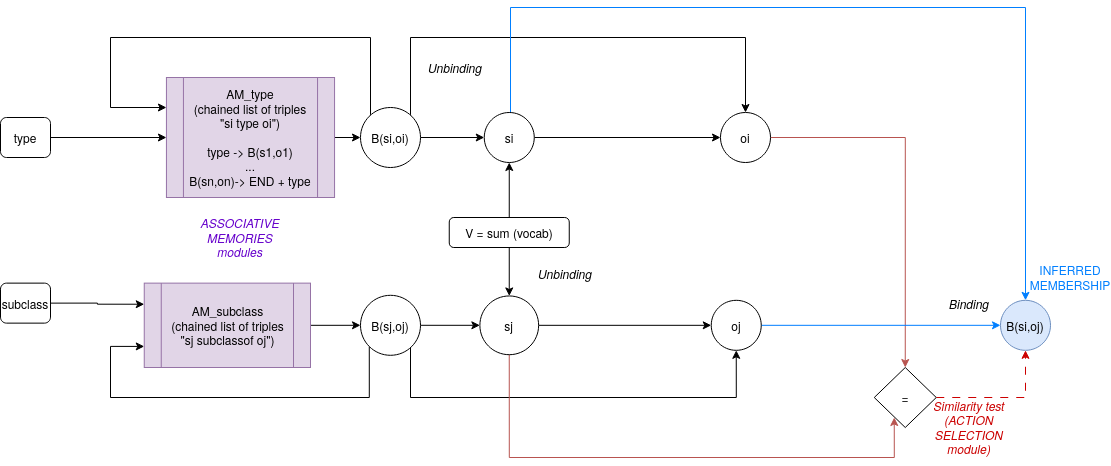
\includegraphics[width=0.9\textwidth]{./architecture_aristotle.png}}
\caption{The Nengo architecture for the class inheritance \textit{rdfs9} forward inference rules; see the text for details. Associative memories storing the relationships are represented by purple rectangles (one for each predicate of interest). We did not represent here the action selection module that triggers the enumeration of the second associative memory, but the one triggering the application of the rule is accounted for by the similarity test explicitized in the red diamond. The rule itself requires the subject and object to be unbound from the retrieved triple; this is done by performing unbinding with the superposition of all semantic pointers from the vocabulary (this is possible thanks to the distributivity of VTB algebra), making it possible to retrieve an isolated vector regardless of what it was bound to. Finally, simply binding the subject $s_j$ to the object $o_i$ makes it possible to infer a new membership (if the gating condition applies), as shown by the blue connections.}
\label{architecture_aristotle}
\end{sidewaysfigure}


Other entailment rules are implemented using similar networks; the associative memories are shared between them, while the enumeration mechanisms are generic, and only the inferred statement is specific to the given rules. The key point is that the whole computing process is distributed and ``programmed'' only by spatial interconnections, as expected.

This shows that our macroscopic implementation can translate to what is proposed to represent biologically plausible processes at a level of representation that can be ``compiled'' as a set of interacting spiking neural networks \cite{eliasmith_how_2013}.

\section{Discussion and conclusion}

\subsection{Contributions}

In this paper, we have been able to propose, up to the implementation level, a reformulation of the powerful VSA approach with a few additions:
\\- We explicitized a degree of belief for each knowledge item that is linked to the possibility theory related to modal logic, and we revisited the main proposed abstraction of biologically plausible data structures to verify their compatibility with this generalization while comparing them with usual programming data structures and discussing how to efficiently scan (i.e., enumerate) such data structures.
\\- We proposed an implementation of hierarchical or relational semantic data structures within the VSA formalism in relation to hierarchical cognitive memory, allowing us to introduce symbolic derivations.
\\- We suggested a design for a forward reasoning mechanism implemented via connectivity feedback on relational data structures, making it possible to perform deductive but also to some extent inductive and abductive reasoning.
\\- We introduced the idea of simulating such a mechanism at a macroscopic, more symbolic level in order to obtain computations independent of the VSA dimension space, thus making it possible to scale up such mechanisms. This idea has been applied to VTB algebra but is also obviously reusable with other VSA algebras.

\subsection{On biological plausibility}

We thus propose an anchoring, i.e., a numerical grounding of semantic information. This, indeed, does not mean that the brain performs such operations exactly, but this anchoring is biologically plausible in the sense that ontology rule-based algorithms can be implemented in a VSA, as developed in this paper, which itself is a model of spiking neuron assembly activity, as developed by \cite{eliasmith_how_2013} with the NEF approach reviewed in this paper.

More technically, we hypothesize that such a neuron assembly stores the ontological assertions (i.e., A-box elements) as a compounded semantic pointer (SPA), while derivations of new assertions (i.e., T-box elements) are implemented as parameterized feedback on this SPA. What we show here is that a general feedback mechanism implements such derivations, while a specific derivation rule corresponds to a specific connectivity of the feedback input layer.
This model implies that new rules are coded by new synapses' long-term connections of feedback connections, thanks to repetitive learning, for instance, due to prefrontal-hippocampus interactions, as modeled by, e.g., \cite{spens_generative_2023}.

This model also implies that assertions are somehow enumerated off-line (in the sense of being scanned and replayed) to infer their consequences, corresponding to forward inference mechanisms (while we discussed a backward mechanism in \cite{mercier_ontology_2021}, such a mechanism is also consistent with prefrontal-hippocampus interactions, as discussed in, e.g., \cite{santos-pata_entorhinal_2021}).

\subsection{On numerical versus semantic grounding}

Numerical grounding, or anchoring, fundamentally differs from the semantic symbol grounding problem, as reviewed and discussed in \cite{taddeo_solving_2005}, where symbols are linked to their meanings and anchored in sensorimotor features, which involves the capacity to pick referents of concepts and a notion of consciousness. In a nutshell, this is still an open problem that we are not going to address here. However, proposals of methods to link abstract symbols to neuronal reality enrich the issue of how mental states can be meaningful. Furthermore, the fact that our abstract representation is anchored in sensorimotor features means that it is also a link between symbols and their potential referents. To take this a step further, when we represent concepts, the chosen design choice associates prototypes, allowing us to anchor an abstract element to a concrete example.

Another aspect not targeted by the present study is the emergence of symbols, i.e., the fact that a symbolic representation emerges from a biological or any physical system in interaction with its environment. This issue corresponds to the ungrounding of concrete signs\footnote{In the semiotic hierarchical meaning of an ``icon'' built only from sensorimotor features, structures at an ``index'' level built by concrete relationships between given objects give rise to a ``symbol'' in the semiotic sense, which corresponds to abstract general relationships between concrete concepts or sensorimotor features.}, as discussed in, e.g., \cite{raczaszek-leonardi_ungrounding_2018}, in relation to the emergence of symbolic thinking (see, e.g., \cite{villiers_why_2007} for a detailed discussion). At the computational neuroscience level, the issue is addressed in \cite{rougier_implicit_2009} for a toy experiment; that paper emphasizes that to address such an issue, we must avoid explicitly embedding any symbol anywhere in the model, a priori or a posteriori. Here, we do not address the emergence issue, but in a sense, we do address a {\em feasibility} issue: To what extent can sophisticated symbolic processing be anchored in numerical processing, not just rudimentary operators? We also address an {\em interpretation} issue, i.e., we consider to what extent sub-symbolic sensorimotor anchored processing corresponds to symbolic processing, as discussed later in this paper.

\subsection{Approach limitations and perspectives}

Although these contributions are of some theoretical and practical interest, it is clear that this is only a preliminary work, far from covering all the modeling and representative power of VSA approaches. It is rather limited regarding several aspects: Although the implementation of inductive and abductive rule-based mechanisms has been evoked and considered, this implementation has not yet been developed. While the RDFS deductive mechanism can clearly be implemented in the present framework, more sophisticated segments of knowledge representation languages such as the OWL 2 family must still be explored to evaluate what can be implemented without extending the present mechanism. Last but not least, another limitation is the fact that, depending on the choice of the entailment rules, an unstable or unbounded number of triples could be generated. This latter caveat can be easily avoided using our knowledge of the different levels of specification of semantic inferences, along with their related decidability and algorithm complexity properties.

The algorithm itself is a simple closure mechanism, although indeed, much more efficient reasoning algorithms are available (such as, e.g., the so-called ``tableau methods''); however, to the best of our knowledge, their link to biologically plausible mechanisms is improbable, whereas we show that a simple set of feedback on iterators does the job and is much closer to what is expected to happen in neural assemblies (see \cite{eliasmith_how_2013} for a general discussion).

The macroscopic simulator is operational but limited to the monotonic entailment rules used in forward mode. We have not yet implemented the capability to delete some rules that could be contradicted by new incoming facts or backward reasoning. Both could be easily implemented as a direct extension of the proposed software package, as described in this paper, but both also require one to make the proper design choices in order for this more general behavior to be coherent.

Following the usual VSA approaches, the symbolic information is embedded in a compact Riemannian manifold with a very simple topology, a hyper-sphere, and we have made explicit the fact that finally, the number of encodable symbols is rather limited. Other geometries may offer better performances, and the particular hyperbolic embedding of hierarchical representations benefits from the fact that due to the hyperbolic negative curvature of the space, even an exponentially growing data structure can be parsimoniously represented \cite{nickel_poincare_2017} because of the expanding geometry (to make a long story short). The idea to embed the data representation in non-Euclidean spaces and especially hyperbolic spaces has already been explored in detail, for instance, in \cite{delahaye_complexites_2006}, showing that the satisfiability and algorithmic complexity can be drastically different\footnote{A version of these elements intended for a wider audience is available in a science popularization journal: \href{https://interstices.info/calculer-dans-un-monde-hyperbolique}..}. This might be an interesting extension of typical VSA approaches that makes it possible to consider the symbol's numerical embedding in such a Riemannian differential manifold. This could be a fruitful perspective of such work.


\backmatter

\bmhead{Acknowledgments}

Terrence C. Stewart is gratefully acknowledged for inspiring advice that helped us with some aspects of this work. Gabriel Doriath Döhler is thanked for his work on clarifying the use of VTB algebra and introducing interesting ideas during his undergraduate internship. Frédéric Alexandre and Hugo Chateau-Laurent are gratefully acknowledged for their valuable advice and their contributions to previous works on this subject. We are especially thankful for the reviewing work on this article, which deeply helped us to make the draft valuable. This work is supported by the \href{Inria, AEx AIDE}{https://team.inria.fr/mnemosyne/en/aide} exploratory action.

\bmhead{Conflict of interest}

This work is not subject to any conflict of interest.

\begin{appendices}

\section{Using VTB algebra} \label{VTB-algebra}

At the mesoscopic level, symbols represent a numerical grounding to real or complex vectors of dimension $d$, with each numerical grounding corresponding to some distributed activity of a spiking neuronal assembly and each algebraic operation corresponding to some transformation of this activity.

Let us review and further develop one of the algebras used to manipulate such symbols at an abstract level in this paper: vector-derived transformation binding (VTB) algebra. We follow \cite{gosmann_vector-derived_2019} and complete the developments in that paper by deriving the different operations at the component level, yielding an optimal implementation and making explicit the computational complexity and related first-order noise. This is in particular used in Appendix~\ref{algorithmic-ersatz} to derive the macroscopic computations.

We consider that $d \defq (d')^2$ for some integer $d'$; thus, it is a quadratic number and we start from the standard definition of the VTB binding operation:
\eqline{\mathbf{z} \defq \mathbf{B_y} \, \mathbf{x},}
where $\mathbf{B_y}$ is a block-diagonal matrix defined as follows:
\eqline{\mathbf{B_y} \defq 
\left[\begin{array}{cccc}
    \mathbf{B_y'} &    0 & \dots &   0 \\
       0 & \mathbf{B_y'} & \dots &    0 \\
    \vdots & \vdots & \ddots & \vdots  \\
       0 &    0 & \dots & \mathbf{B_y'}
    \end{array}\right],
\mbox{ with } 
\mathbf{B_y'}  \defq \sqrt{d'} \,
\left[\begin{array}{cccc}
    y_1            & y_2            & \dots  & y_{d'}  \\
    y_{d' + 1}     & y_{d' + 2}     & \dots  & y_{2d'} \\
    \vdots         & \vdots         & \ddots & \vdots  \\
    y_{d - d' + 1} & y_{d - d' + 2} & \dots  & y_d
\end{array}\right],}
or equivalently\footnote{All algebraic derivations reported here are straightforward and were verified using a piece of symbolic algebra code available at \url{https://raw.githubusercontent.com/vthierry/onto2spa/main/figures/VTB-algebra.mpl}.}, for $i = 1 \cdots d$,
\begin{equation}\label{eq-binding}
  \left\{\begin{array}{rcl}
      [\mathbf{z}]_i \defq \mathbf{B_y} \, \mathbf{x} &=& \sqrt{d'} \, \sum_{k = 1}^{k = d'} [\mathbf{y}]_{k + \beta(i)} \; [\mathbf{x}]_{k + \alpha(i)}, \\
      \left[\mathbf{B_y}\right]_{ij} &=& \sqrt{d'} \, \delta_{i \le d' \mbox{ and } j \le d'} [\mathbf{y}]_{k + \beta(i) - \alpha(i)}, \\
  \end{array}\right.
\mbox{written} \left\{\begin{array}{rcl} 
  \alpha(i) &\defq& d' \, ((i-1) \mbox{ div } d'), \\
  \beta(i)  &\defq& d' \, ((i-1) \mbox{ mod } d'), \\
\end{array}\right.
\end{equation}
with the matrix multiplication explicitized as a sum, which can be easily verified. Here, $[\mathbf{z}]_k$ stands for the k-th coordinate of the vector $\mathbf{z}$, and $\delta_{\cal P}$ is $1$ if ${\cal P}$ is true; otherwise, it is $0$. This is our basic definition, and reformulating the VTB operation using~(\ref{eq-binding}) will allow us to better understand its properties.

This operation is bi-linear in $\mathbf{x}$ and $\mathbf{y}$, and thus it is distributive with respect to addition and the scalar product.

The $\sqrt{d'}$ renormalization factor allows $\mathbf{z}$ to have a unary magnitude\footnote{More precisely, two random normalized vectors of dimension $d$ drawn from a random normal distribution of independent samples verify that ${\bf x} \cdot {\bf y} \sim {\mathcal N}(0, 1/d')$, as described in subsection~\ref{symbol-encoding}. Then, applying a permutation on all indices on a random vector $\mathbf{x}$ yields another random vector, which is not correlated with any vector $\mathbf{y}$ if $\mathbf{x}$ is not. Thus, when computing the components $[\mathbf{z}]_i$ in (\ref{eq-binding}) for two general random vectors $\mathbf{x}$ and $\mathbf{y}$, we compute the dot product of two random vectors of dimension $d'$ renormalized by $\sqrt{d'}$, and thus this dot product comes from the distribution ${\mathcal N}(0, 1)$; this corresponds to drawing a random vector unary on average.}.

At the algorithmic implementation level, the calculation of $\mathbf{z}$ is performed in\footnote{Each of the $d$ components  $[\mathbf{z}]_i$ requires a dot product of size $d' = \sqrt{d}$ that is not factorizable in the general case, since involving different elements of the vectors as readable on the matrix form.} $O\left(d^{\frac{3}{2}}\right)$ operations, and the $\mathbf{y}_{k + \beta[i]}$ and $\mathbf{x}_{k + \alpha[i]}$ indexing can be tabulated in two fixed look-up tables $\beta[i]$ and $\alpha[i]$, avoiding any additional calculations. Furthermore, the fact that $\sqrt{d'}$ is an integer makes it possible to limit numerical approximations in order to improve numerical conditioning. This will be verified for all other explicit formulae later in this paper.
We make explicit these formulae in detail not to re-implement these operations, which are already available in the Nengo simulator, but to study in detail their complexity and their precision, with the goal of proposing a macroscopic algorithmic ersatz of these operations.

This can be compared to the fastest binding operation, which is convolution implemented via the fast Fourier transform \cite{schlegel_comparison_2020}, and thus it has a complexity of $O\left(d\, \log(d)\right)$:
\\\centerline{\begin{tabular}{|l|c|c|c|c|}
\hline
            & d = 10     & d = 100    & d = 500   & d = 1000  \\
\hline
VTB         & $10^{1.5}$  & $10^3$     & $10^4$    & $10^{4.5}$ \\
\hline
Convolution & $10^{1.4}$  & $10^{2.6}$  & $10^{3.5}$ & $10^{3.8}$ \\
\hline
Ratio $=\frac{\sqrt{d}}{\log(d)}$ & $\simeq 1$ & $\simeq 2$ & $\simeq 3.5$ & $\simeq 4.5$ \\
\hline
\end{tabular}} \\

As stated in \cite{gosmann_vector-derived_2019} and reviewed in \cite{mercier_ontology_2021}, the key point is that this binding operation generates a new vector $\mathbf{z}$ that is almost orthogonal to $\mathbf{x}$ and $\mathbf{y}$:
\eqline{(\mathbf{B_y} \, \mathbf{x}) \cdot \mathbf{x} \simeq 0,}
and this operation is neither commutative,
\eqline{(\mathbf{B_x} \, \mathbf{y}) \cdot (\mathbf{B_y} \, \mathbf{x}) \simeq 0,}
nor associative\footnote{Of course, as a product of matrices, the combination of three bindings or two binding operations and a vector is associative, but the operator $\mathbf{B}$ itself is not, as made explicit in the formula.}, in the following sense:
\eqline{(\mathbf{B_{(B_z \, y)}} \, \mathbf{x}) \cdot ((\mathbf{B_z} \, \mathbf{B_y}) \, \mathbf{x}) \simeq 0.}
These properties ensure that we do not infer spurious derivations.

To take this a step further, in the real case, the random matrix is almost orthogonal, i.e.,
\eqline{\mathbf{B_y^\top} \, \mathbf{B_y} \simeq \mathbf{I},}
for the same reasons evoked above. It is straightforward to evaluate the precision of this approximation, which is again in ${\mathcal N}(0, O(1/d'))$ for each matrix element\footnote{From~(\ref{eq-binding}), we derive
\eqline{\begin{array}{rcl}
    \left[\mathbf{B_y^\top} \, \mathbf{B_y}\right]_{ij}
    &=& \sum_{k = 1}^{d'} [\mathbf{B_y}]_{ki} \, [\mathbf{B_y}]_{kj} \\
    &=& d' \, \sum_{k = 1}^{d'} [\mathbf{y}]_{k + \beta(i) - \alpha(i)} \, [\mathbf{y}]_{k + \beta(j) - \alpha(j)} \\
    &=& d' , \sum_{l = 1}^{d'} [\mathbf{y}]_l \, [\mathbf{y}]_{k + (\beta(j) - \beta(i)) - (\alpha(j) - \alpha(i))} \\
    &=& d' , \sum_{l = 1}^{d'} [\mathbf{y}]_l \, [\mathbf{y}]_{k + d' \, ((j - i) \mbox{ div } d') - ((j - i) \mbox{ div } d')}, \\
\end{array}}
so that
\\- $\left[\mathbf{B_y^\top} \, \mathbf{B_y}\right]_{ii} = \sum_{l = 1}^{d'} [\mathbf{y}]_l^2 = 1 + {\mathcal N}(0, O(1/d'))$, as derived in subsection~\ref{symbol-encoding}; and
\\- $\left[\mathbf{B_y^\top} \, \mathbf{B_y}\right]_{ij, i \ne j} = {\mathcal N}(0, O(1/d'))$, because it is easy to verify that $((j - i) \mbox{ div } d') - ((j - i) \mbox{ div } d') \ne 0$ when $i \ne j$, so that the dot product of $d'$ random components of $[\mathbf{y}]_l$ with $d'$ other random components yields normal noise, as made explicit in subsection~\ref{symbol-encoding}.}. This also means that the level of noise is relatively high, $O\left(\frac{1}{d^{\frac{1}{4}}}\right)$ instead of $O\left(\frac{1}{d^{\frac{1}{2}}}\right)$, which explains the relatively limited numerical performances of simulations with $d< 10^3$, as reported, for instance, in \cite{schlegel_comparison_2020}.


We thus define
\eqline{\mathbf{B_{y^\sim}} \defq \mathbf{B_y^\top} \mbox{ with } [\mathbf{y^\sim}]_i \defq [\mathbf{y}]_{\sigma(i)},}
with
\eqline{\sigma(i) \defq  1 + d' \, ((i-1) \mbox{ mod } d') + (i-1) \mbox{ div } d'.}
In other words, $\mathbf{B_y^\top}$ has the same structure as $\mathbf{B_y}$, except that the vector coordinates are subject to a permutation $\sigma(i)$, which is idempotent ($\sigma(\sigma(i)) = i$) and thus its own inverse, so that if 
$\mathbf{z'} \defq \mathbf{B_{y^\sim}} \, \mathbf{x}$, we obtain
\eqline{[\mathbf{z'}]_i = \sqrt{d'} \, \sum_{k = 1}^{k = d'} [\mathbf{y}]_{\sigma(k + \beta(i))} \; [\mathbf{x}]_{(k + \alpha(i))}} (where $\beta(i)$ and $\alpha(i)$ are the indexing defined to calculate $\mathbf{B_{y}} \, \mathbf{x}$ explicitly), and this makes it possible to define a left unbinding operation:
\eqline{\mathbf{B_{y^\sim}} \, (\mathbf{B_y} \, \mathbf{x}) = \mathbf{B_y^\top} \, \mathbf{B_y} \, \mathbf{x}
  = \mathbf{x} + {\mathcal N}(\mathbf{0}, O(1/d)) \simeq \mathbf{x}.}
 Thus, again, this results in additive noise of $O(1/d^{1/4})$.

The right identity vector $\mathbf{\mathbf{i}}$ such that $\mathbf{B_{\mathbf{i}}} = \mathbf{I}$ can be written explicitly as follows:
\eqline{[\mathbf{\mathbf{i}}]_i = \frac{1}{\sqrt{d'}} \, \delta_{i = \sigma(i)}.}
In other words, we get $i_B$ by ``unfolding'' the identity matrix $I_d'$ line by line, writing a $1$, then $d$ times $0$, then another $1$, and so on.

Considering the mirroring matrix $\mathbf{B_{\leftrightarrow}}$, which is defined as
\eqline{[\mathbf{B_{\leftrightarrow}}]_{ij} \defq \delta_{j = \sigma(i)}}
(which is thus not block-diagonal in the way that a matrix of the form $\mathbf{B_y}$ is), so that $\mathbf{B_{\leftrightarrow}} \, \mathbf{x} = \mathbf{x}^\sim$, we obtain
\eqline{\mathbf{B_{\leftrightarrow}} \, \mathbf{B_y} \, \mathbf{x} = \mathbf{B_x} \, \mathbf{y},
\mbox{ while } \mathbf{B_{\leftrightarrow}} \,\mathbf{B_{\leftrightarrow}} = \mathbf{I} \mbox{ and } \mathbf{B_{\leftrightarrow}^\top} = \mathbf{B_{\leftrightarrow}},}
which makes it possible to define a right unbinding operation:
\eqline{(\mathbf{B_{x^\sim}} \, \mathbf{B_{\leftrightarrow}}) \, (\mathbf{B_y} \, \mathbf{x}) = \mathbf{B_{x^\sim}} \, \mathbf{B_x} \, \mathbf{y} \simeq \mathbf{y}.}

Unfortunately, $\mathbf{B_{\leftrightarrow}}$ is not a binding matrix, i.e., it is not of the form $\mathbf{B_z}$ for some vector $\mathbf{z}$, which is easily verified by the fact that some components that must be equal to $0$ for a binding matrix are equal to $1$ in $\mathbf{B_{\leftrightarrow}}$. Furthermore, the left or right multiplication of a binding matrix by this mirroring matrix does not yield a binding matrix, because of the same observation; components that must be equal to $0$ for a binding matrix are equal to $1$ in $\mathbf{B_{\leftrightarrow}}$.

Beyond \cite{gosmann_vector-derived_2019}, the authors of \cite{mercier_ontology_2021} introduced a vector composition operator $\oslash$ to make explicit the composition of two binding operations, namely,
\eqline{\mathbf{B_v} = \mathbf{B_y} \, \mathbf{B_x} \Leftrightarrow \mathbf{v} \defq \mathbf{y} \oslash \mathbf{x},}
which can be explicitly written as follows\footnote{Since $\mathbf{B_y}$ and $\mathbf{B_x}$ are block-diagonal matrices, it is easy to verify that $\mathbf{B_v}$ is a block-diagonal matrix with a $d' \times d'$ block $\mathbf{B_v}' = \mathbf{B_y}' \, \mathbf{B_x}'$ using the notation from the beginning of this section, and we can explicitly write that
\eqline{[\mathbf{B_v}']_{ij} = \sqrt{d'} \, \sqrt{d'} \, \sum_{k = 1}^{d'} [\mathbf{y}]_{k + (i - 1) \mbox{ div } d'} \, [\mathbf{x}]_{(k - 1) \, d' + j},}
from which we obtain the desired formula.}:
\eqline{[\mathbf{v}]_i = \sqrt{d'} \, \sum_{k = 1}^{k = d'} [\mathbf{y}]_{(i - 1) \, d' + k} \, [\mathbf{x}]_{1 + d' \, (k - 1) + (i - 1) \mbox{ mod } d'}.} At the algebraic level, the key point is that the product of two binding matrices is still a binding matrix. As a consequence, this composition operator is bi-linear, and thus it is distributive with respect to addition; it is not commutative, but it is associative and commutes with the inversion as follows:
\eqline{(\mathbf{y} \oslash \mathbf{x})^\sim = \mathbf{x}^\sim \oslash \mathbf{y}^\sim,}
while $\mathbf{x}^\sim \oslash \mathbf{x} \simeq \mathbf{\mathbf{i}}$; all these results can be easily derived by considering usual matrix properties. This allows us to combine two binding matrices without an explicit matrix product in $O\left(d^{\frac{3}{2}}\right)$ operations only. At the numeric level, since $\mathbf{v}$ is up to a $\sqrt{d'}$ factor, the dot product of segments of random vectors of dimension $d'$ follows a normal distribution of standard deviation $O(1/d')$. We also find that
\eqline{[\mathbf{v}]_i = {\mathcal N}(\mathbf{0}, O(1/d'^2)),}
which is a rather high level of noise, when an unbinding operation is applied, for instance, to an associative map.

\subsection*{Using VTB algebra in the complex case}

All of the developments described in this section generalize to complex numbers. Although it is not directly used here, such a generalization is of general interest because complex implementations of VSA frameworks have also been considered \cite{schlegel_comparison_2020}. Furthermore, it is also of interest to see if our macroscopic implementation could be easily adapted to the complex case.

Stating that two resources are semantically equivalent if the unary vectors are aligned can be written in the complex case as follows\footnote{If we are in the real case $\mathbf{x}$ and $\mathbf{y} \in {\mathcal R}^d$, with $\|{\bf x}\|_2 = \|{\bf y}\|_2 = 1$, then the equality is written as \eqline{\mathbf{x} = \mathbf{y} \Leftrightarrow \mathbf{x} \cdot \mathbf{y} = \sum_i x_i \, y_i = \cos\left(\widehat{\overrightarrow{\mathbf{x}} \, \overrightarrow{\mathbf{y}}}\right) = 1 \Leftrightarrow \widehat{\overrightarrow{\mathbf{x}} \, \overrightarrow{\mathbf{y}}} = 0 \; (\mbox{mod} \; 2 \, \Pi),}
i.e., both unary vectors have the same direction; in other words, they are aligned.
If we are in the complex case $\mathbf{x}$ and $\mathbf{y} \in {\mathcal C}^d$, let us consider the canonical embedding in ${\mathcal R}^{2\,d}$, i.e., we consider the real ($Re$) and imaginary ($Im$) parts as two real coordinates, denoting by $\overrightarrow{\mathbf{x}}$ the corresponding vector:
\eqline{\mathbf{x} \defq \left(x_1, x_2, \cdots \right)^T \Leftrightarrow \overrightarrow{\mathbf{x}} \defq \left(Re(x_1), Im(x_1), Re(x_2), Im(x_2), \cdots\right)^T,}
where $z^*$ is the conjugate of a complex number $z$, while $<\mathbf{x} \vert \mathbf{y}>$ stands for the complex inner product:
\eqline{\begin{array}{rcl}<\mathbf{x} \vert \mathbf{y}> 
&\defq& \sum_i x_i \, y_i^* \\
&=& \sum_i 
  (Re(x_i) \, Re(y_i) + Im(x_i) \, Im(y_i)) + I \, (Re(x_i) \, Im(y_i) - Im(x_i) \, Re(y_i)) \\
&=&
  \overrightarrow{\mathbf{x}} \cdot \overrightarrow{\mathbf{y}} + I \, 
  \overrightarrow{\mathbf{x}}^* \cdot \overrightarrow{\mathbf{y}},
\end{array}}
so that $Re(<\mathbf{x} \vert \mathbf{y}>) = \overrightarrow{\mathbf{x}} \cdot \overrightarrow{\mathbf{y}}$ and $\|\mathbf{x}\| = \sqrt{<\mathbf{x} \vert \mathbf{x}>} = \|\overrightarrow{\mathbf{x}}\|-2 = \sqrt{\overrightarrow{\mathbf{x}} \cdot \overrightarrow{\mathbf{x}}}$, and since vectors are unary, 
\eqline{<\mathbf{x} \vert \mathbf{y}> = 1 \Leftrightarrow \overrightarrow{\mathbf{x}} \cdot \overrightarrow{\mathbf{y}} = 1 \Leftrightarrow \overrightarrow{\mathbf{x}} = \overrightarrow{\mathbf{y}} \Leftrightarrow \mathbf{x} = \mathbf{y},}
making explicit the obvious fact that unary real or complex vectors are equal if and only if their inner product equals one, while we consider the ``angle'' of two complex vectors as the angle of their $2\,d$ real embedding, i.e.,
\eqline{\widehat{\mathbf{x} \, \mathbf{y}} \defq \mbox{arccos}(Re(<\mathbf{x} \vert \mathbf{y}>)).}}: 
\eqline{\mathbf{x} \simeq \mathbf{y} \Leftrightarrow <\mathbf{x} \vert \mathbf{y}> \simeq 1,
% https://mathcs.clarku.edu/~ma130/inner2.pdf
} while the orientation is usually defined as
\eqline{\widehat{\mathbf{x} \, \mathbf{y}} \defq \mbox{arccos}(Re(<\mathbf{x} \vert \mathbf{y}>)),}
as explained in the previous footnote.

Provided that the space dimension $d$ is large enough, two randomly chosen different complex vectors $\mathbf{x}$ and $\mathbf{y}$\footnote{
Considering again the canonical embedding in ${\mathcal R}^{2\,d}$ and the fact that
\eqline{<\mathbf{x} \vert \mathbf{y}> = \overrightarrow{\mathbf{x}} \cdot \overrightarrow{\mathbf{y}} + I \, 
  \overrightarrow{\mathbf{x}^*} \cdot \overrightarrow{\mathbf{y}},}
because $\overrightarrow{\mathbf{x}}$ and thus $\overrightarrow{\mathbf{x}}^*$ and $\overrightarrow{\mathbf{y}}$ are random vectors, their dot product almost vanishes; thus, the real and imaginary parts of $<\mathbf{x} \vert \mathbf{y}>$ also almost vanish.} will also be approximately orthogonal in the sense that
\eqline{\mathbf{x} \neq \mathbf{y} \Leftrightarrow <\mathbf{x} \vert \mathbf{y}> \simeq 0.}
As a consequence, the VTB matrix is almost a unitary matrix, i.e., 
\eqline{\mathbf{B_y}^* \, \mathbf{B_y} \simeq \mathbf{I},}
considering the conjugate transpose.

All other algebraic operations are common to both real and complex linear algebra, and this is also the case for other VSA binding operators.

More than just a confirmation, these derivations allow us to observe that using a complex representation would be interesting if the conjugate of a vector could have a semantic interpretation. In that case, if, say, $\mathbf{x}$ and $\mathbf{y}^*$ are similar, then $<\mathbf{x} \vert \mathbf{y}> \simeq I$, as easily verified from the previous derivations. 

\section{On VSA data structures} \label{data-structure}

This section revisits the literature, emphasizing the properties of the data structures; it discusses in more detail their computational properties and limitations and links them to usual programming language data structures.

\subsection{Unordered set or bundling}

We first consider an unordered set ${\cal S}$ of $N$ symbols grounded to values $\{\mathbf{s}_1, \cdots \mathbf{s}_i \cdots \mathbf{s}_N\}$, and we would like to be able to store them in such a way that we can check if a given symbol is in the set. Very simply, we ground ${\cal S}$ to the vector $\mathbf{s}$:
\eqline{\mathbf{s} \defq \sum_i \mathbf{s}_i,}
which provides a solution, because given a symbol $\mathbf{s}_\bullet$, we obviously observe that $\mathbf{s}_\bullet \cdot \mathbf{s} \simeq 1$ if it corresponds to a certain symbol $\mathbf{s}_i$, and it is almost $0$ otherwise, because random vectors are almost orthogonal, as previously explained. This is called bundling \cite{schlegel_comparison_2020} or superposition.

Furthermore, the representation intrinsically includes a notion of transitivity: If a set includes another subset, by construction, it includes the subset elements. More precisely,
\eqline{\mathbf{s} \defq \sum_i \mathbf{s}_i \mbox{ and } \mathbf{s}_i \defq \sum_j \mathbf{s}_{ij} \Rightarrow \mathbf{s} \defq \sum_{ij} \mathbf{s}_{ij},}
and thus, $\mathbf{s}_{ij} \cdot \mathbf{s} > 0$ for all subset elements.

This obviously generalizes to weighted symbols $\hat{\mathbf{s}}_i$, i.e., symbols with modality weighting. In that case, $\mathbf{s}_\bullet \cdot \mathbf{s} \simeq \tau$ makes it possible to retrieve the belief weight. This is equivalent to inputting a symbol $\mathbf{s}_\bullet$ that is approximately similar to a given symbol $\mathbf{s}_i$, thus indicating an approximate similarity; however, it neither allows us to retrieve the exact value of $\mathbf{s}_i$ nor indicates if a positive value below $1$ corresponds to a weighted symbol that has been exactly retrieved or to a symbol approximation.

This has an interesting biological interpretation: ${\cal S}$ has features in common with a Hopfield network or other related attractor networks, where information has been stored in a distributed way while activating the map with an input makes it possible to determine whether the symbol is stored or not. The main difference is that attractor networks converge to the exact stored value, providing a mechanism of associative memory, which is now developed while introducing superposition, allowing us to better understand the need for a more sophisticated mechanism.

Let us provide an analogy with programming data structures, explicitizing the similarities and differences between what is proposed here and what is available in common programming languages\footnote{We will do the same for other cognitive structures because we think that it illustrates the computing capability of the cognitive object.}. This unordered set representation corresponds to a ``set'' container (e.g., a {\tt std::unordered\_set} in C++ or a {\tt set()} in Python) that has only an insertion method and a membership test function, without the capability to intrinsically enumerate the elements, as formerly discussed.

\subsubsection{Symbol enumeration}

At this stage, this structure does not allow us to directly enumerate all symbols $\mathbf{s}_i$, because from $\mathbf{s}$, it is not possible to decode the superposed vectors. In \cite{crawford_biologically_2016}, for instance, where data structures are defined using superposition, the intrinsic memory enumeration of the stored information is not addressed. We thus need an external mechanism to select all elements and perform an operation on each one. However, at the implementation level, in Nengo \cite{eliasmith_how_2013}, an explicit list of the defined vocabulary $\{\cdots \mathbf{s}_i \cdots\}$ is maintained, and the way to select the elements is to test $(\mathbf{s}^T \, \mathbf{s}_i)$ for each element of the vocabulary. This select operator has a complexity of $O(K)$, where $K$ is the size of the vocabulary. Later in this paper, we will also propose a biologically plausible indexing mechanism, in order, for instance, to manipulate sequences.

\subsection{Associative map}

We now consider an unordered associative memory\footnote{This is not the only way to implement such an associative memory: In \cite{voelker_learning_2014}, binding/unbinding is not explicitly used, and an input/output architecture with suitable connections is used instead. Each input unit has an encoding vector in which input weights are tuned to fire for a specific key and drive a connected output vector that is optimized to estimate the value associated with the related key.}, or ``map,'' of $N$ correspondences $\{\mathbf{s}_1 \rightarrow \mathbf{o}_1, \cdots \mathbf{s}_i \rightarrow \mathbf{o}_i \cdots \mathbf{s}_N \rightarrow \mathbf{o}_N\}$ between subjects and objects. To this end, we use the binding operation $B_{\mathbf{s}_i}$, defined in Appendix~\ref{VTB-algebra},  with a pseudo-inverse, i.e., an unbinding operator, $B_{\mathbf{s}_i^\sim}$:
\eqline{\mathbf{m} \defq \sum_i B_{\mathbf{s}_i} \, \mathbf{o}_i,}
so that
\eqline{B_{\mathbf{s}_\bullet^\sim} \, \mathbf{m} \simeq \sum_{i, \mathbf{s}_\bullet = \mathbf{s}_i} \mathbf{o}_i.}
In other words, the unbinding operation makes it possible to retrieve the set, i.e., the additive superposition of all objects $\mathbf{o}_i$ associated with a given subject $\mathbf{s}_\bullet$, while $B_{\mathbf{s}_k^\sim} \, {\cal S} \simeq 0$ if none. This is done up to a level of noise of $O(1/d^{1/4})$, as derived in Appendix~\ref{VTB-algebra}, which is rather high with respect to the similarity precision, which is $O(1/d^{1/2})$, as observed numerically \cite{schlegel_comparison_2020}; however, in biological neuronal networks, where the dimension is an order of magnitude higher, this is no longer a limitation because $d$ is high. 

This allows us to detect if the information is in the table and retrieve this information in one step if this is the case. However, as in the previous case, no mechanism allows the enumeration of the map subjects or objects.

This algebraic construction also makes it possible to retrieve the subjects associated with a given object, because of the commutator $\mathbf{B_{\leftrightarrow}}$, such that
\eqline{\mathbf{B_{\leftrightarrow}} \, \mathbf{B}_{\mathbf{o}_i} \, \mathbf{s}_i = \mathbf{B}_{\mathbf{s}_i} \, \mathbf{o}_i,}
yielding
\eqline{\mathbf{m_{\leftrightarrow}} \defq \mathbf{B_{\leftrightarrow}} \, \mathbf{m} = \sum_i B_{\mathbf{o}_i} \, \mathbf{s}_i,}
which is now the numerical grounding of the reciprocal map $\{\mathbf{o}_1 \rightarrow \mathbf{s}_1, \cdots \mathbf{o}_i \rightarrow \mathbf{s}_i \cdots \mathbf{o}_N \rightarrow \mathbf{s}_N\}$.

The algebraic construction also offers the notion of the identity vector $\mathbf{i}$, with $\mathbf{B_{\mathbf{i}}} = \mathbf{I}$, so that
\eqline{\mathbf{s}_i = \mathbf{i} \rightarrow B_{\mathbf{s}_i} \, \mathbf{o}_i = \mathbf{o}_i.}
In other words, the binding reduces to a superposition. Theoretical details underlying the implementation of such associative memories are available in \cite{stewart_biologically_2011}.

As for the previous structure, this obviously generalizes to weighted symbols $\hat{\mathbf{s}}_i$ and an approximate input
$\mathbf{s}_\bullet \simeq \hat{\mathbf{s}}_i$, allowing us to retrieve the object $\mathbf{o}_i$ weighted by either the modality weighting or the input approximation, indistinctly.

There are several solutions used to define such binding, unbinding, and commutator operators. A proposed solution is developed in Appendix~\ref{VTB-algebra} after the work in \cite{gosmann_vector-derived_2019}, which was completed by \cite{mercier_ontology_2021}. This design choice is guided by the fact that we need to avoid spurious inferences: With a commutative operator (such as the convolution operator), $\mathbf{B}_{\mathbf{o}_i} \, \mathbf{s}_i$ would equal $\mathbf{B}_{\mathbf{s}_i} \, \mathbf{o}_i$, which could generate nonsense deductions (e.g., for a driver-vehicle map, this would mean that if Ming-Yue drives a bicycle, then the bicycle drives Ming-Yue unless some additional mechanism is considered to avoid such nonsense). The proposed VTB algebra avoids such caveats (see \cite{schlegel_comparison_2020} for a recent comparison of different VSAs)\footnote{An alternative to VTB algebra is called MBAT algebra; it requires matrix inversion instead of transposition, and thus it is less efficient.}. 

This associative memory mechanism has an interesting biological interpretation: It implements an associative memory in the biological sense, with the association stored in a distributed way, and activating the associative memory with an input $\mathbf{s}_\bullet$ allows us to retrieve the associated symbol. This is what happens in several biological mechanisms, as reviewed, for instance, in \cite{eichenbaum_memory_2017}. 

In particular, a structure of the form
\eqline{\mathbf{m} \defq \sum_n B_{\mathbf{s}_i} \, \mathbf{s}_i}
that maps an object onto itself allows the retrieval of an exact symbol from an approximate input, solving the caveats induced by using only a superposition mechanism that was presented previously. This is exactly what is expected in an associative encoder (e.g., a Hopfield network); if a symbol is close to an existing symbol, the associative memory will output a weighted version of the symbol.

At the computer programming level, this corresponds to a ``map'' container (e.g., a {\tt Map} in JavaScript or a {\tt dictionary()} in Python), again with only insertion and retrieval methods, and without intrinsic iterators.

To take this a step further, we can propose a complementary functionality, defining an additional symbol ``something'' whose numerical grounding is fixed to any new random vector $\mathbf{\sigma}$ that is never used elsewhere. This allows us to enhance the information to be obtained as follows: Each time a piece of information $\mathbf{s}_i \rightarrow \mathbf{o}_i$ is added, we also add $\mathbf{s}_i \rightarrow \mathbf{\sigma}$  and $\mathbf{\sigma} \rightarrow \mathbf{o}_i$, i.e., we make explicit the fact that $\mathbf{s}_i$ and $\mathbf{o}_i$ are defined in this table, which can be retrieved in one step, without the need to enumerate the different elements. In such a case,
\eqline{\mathbf{m}_{\mathbf{s}_j} \defq \sum_{i, \mathbf{s}_j = \mathbf{s}_i} \mathbf{o}_i = P_{\mathbf{\sigma}^\perp} \,  B_{\mathbf{s}_i^\sim} \, \mathbf{m},}
where $P_{\mathbf{\sigma}^\perp} \defq \mathbf{I} - \mathbf{\sigma} \, \mathbf{\sigma}^T$ is the projection onto the orthogonal of $\mathbf{\sigma}$, i.e., we must eliminate the symbol ``something'' from the expected values.

\subsection{Indexed and chained list}

\subsubsection{Construction of indexes}

In order to define an indexed list, we need indexes, i.e., a mechanism that generates ordinal values. Our main purpose here is to make explicit that what has been developed using convolution operators \cite{komer_neural_2019} still holds with VTB. We fix the symbol grounding of the ``zero'' symbol $\mathbf{\nu}_0$, which is never used elsewhere, and define the following recursively:
\eqline{\mathbf{\nu}_{n + 1} \defq B_{\mathbf{\nu}_0} \, \mathbf{\nu}_n,}
i.e., the $(n+1)$-th ordinal value is obtained by binding the $n$-th, and we easily obtain, from a few algebra operations,
\eqline{B_{\mathbf{\nu}_p} \, \mathbf{\nu}_q = B_{\mathbf{\nu}_q} \, \mathbf{\nu}_p = B_{\mathbf{\nu}_{p+q}} \, \mathbf{\nu}_0, \;\;\; 
B_{\mathbf{\nu}_p} \, \mathbf{\nu}_q^\sim = B_{\mathbf{\nu}_q^\sim} \, \mathbf{\nu}_p  \simeq B_{\mathbf{\nu}_{p-q}} \, \mathbf{\nu}_0.}
In particular, $\mathbf{\nu}_{n - 1} \simeq B_{\mathbf{\nu}_0^\sim} \, \mathbf{\nu}_n$, so that the definition
holds for $n \in {\cal Z}$.

Here, we only consider the minimal material needed to build an indexed list; numerical information in the brain is a much more complex subject \cite{nieder_representation_2007} beyond the scope of this work.

\subsubsection{Indexed list} 
We can now define an indexed list or array, often called a vector, since the previous mechanism allows us to generate a ``counter'' that can be incremented or decremented using the binding or unbinding operator.

To this end, an associative map indexed by these ordinals can be managed as a list whose values can be enumerated. Such a representation is also present at several cognitive levels when considering temporal sequences, actions, or any enumeration. This is also the tool that allows us to enumerate all elements of a symbol set ${\cal S}$, which was defined previously, or the subjects of an associative map.

To make this mechanism explicit, let us consider a list $\mathbf{l} \defq \sum_i B_{\mathbf{\nu}_i} \, \mathbf{l}_i$, and a variable index $\mathbf{k}$. A construct of the form
\begin{algorithmic}
  \For{$\mathbf{k} \leftarrow \mathbf{\nu}_0 $;
    {\bf while} $\|B_{\mathbf{k}} \, \mathbf{l}\| > 0$;
    {\bf next} $\mathbf{k} \leftarrow B_{\mathbf{\nu}_0} \, \mathbf{k}$}
   \State $\mathbf{l}_i \leftarrow B_{\mathbf{k}^\sim} \, \mathbf{l}$
\State ../..
\EndFor
\end{algorithmic}
allows us to enumerate\footnote{In fact, considering $\mathbf{l} \defq \sum_i B_{\mathbf{\nu}_i} \, \mathbf{l}_i + B_{\mathbf{\nu}_{-1}} \, \lambda$, where $\lambda$ is the list length, which is updated when an element is added or deleted, would improve the algorithmic ersatz implementation, which is not the issue here.} all elements, this being indeed only an algorithmic ersatz to illustrate the mechanism beyond the biologically plausible implementation of sequential memory organization.

At the biological plausibility level, following \cite{eichenbaum_memory_2017}, we may consider that the brain can have three kinds of memory: associative, sequential, and hierarchical (called schematic by the author of \cite{eichenbaum_memory_2017}) memory. All three memory types are present and required for cognitive processes. The VSA approach provides both associative and sequential memory. Let us consider the third type of memory, which has not, to the best of our knowledge, been addressed with regard to VSAs.

At the computer programming level, this corresponds to an extensible ``array'' (e.g., a {\tt std::vector} in C++ or {\tt java.util.AbstractList} in Java), with basic edition and retrieval methods available.

\subsubsection{Chained list}

We can also define a chained list using an associative memory of the form
  \eqline{\begin{array}{rcl}
      \mbox{\tt first} &\rightarrow& \mbox{\tt second} \\
      \mbox{\tt second} &\rightarrow& \mbox{\tt third} \\
      \cdots & \\
      \mbox{\tt last} &\rightarrow& \mbox{\tt END + first}
    \end{array},}
where every value of the list acts as a key to the value of its successor in the list, thus enumerating the values. {\tt END} is a predefined specific symbol that makes it possible to know when the list ends that we can superpose to a pointer to the first value in case we need to iterate through the entire list again.

We also could have considered multiple binding\footnote{In such a case, a list of the form $l = [v_1, v_2, \cdots]$ is encoded without associative memory as \eqline{\mathbf{l} = B_{\mbox{\tt value}} \, \mathbf{v}_1 + B_{\mbox{\tt next}} \, \left(B_{\mbox{\tt value}} \, \mathbf{v}_2 + B_{\mbox{\tt next}}\left(\cdots + B_{\mbox{\tt next}}\left(\mbox{\tt list-end}\right)\right)\right),}
allowing us to obtain by unbinding the list's head value and its tail value, and allowing us to detect its end. This corresponds, for instance, to the {\tt rdf:first}, {\tt rdf:rest}, and {\tt rdf:nil} symbols of the RDF representation. However, as discussed in Appendix~\ref{VTB-algebra}, chaining unbinding operations is not numerically very robust due to the additional residual noise.}, as proposed in \cite{mercier_ontology_2021}.
 
\section{RDFS entailment rules implementation} \label{RDFS-entailment-rules}

As a side product of the present development, we would like to illustrate the computational capability of the proposed framework by briefly showing that our biologically plausible mechanism is at least able to perform RDFS\footnote{This is true according to the \url{https://www.w3.org/TR/rdf-schema} specification.} specification inferences. This is done, of course, without any assumption about the fact that the brain explicitly performs such computations\footnote{Considering knowledge representation and reasoning, the capabilities of semantic web modeling languages, such as RDFS and Web Ontology Language (OWL) (see, e.g., \cite{allemang_semantic_2020} for a recent didactic reference), make them a powerful way to solve modeling problems and manipulate high-level data representations. They also appear to be rather accessible to an educated person, as pointed out in \cite{allemang_semantic_2020}, and correspond in part to the usual common-sense formalization, for instance, in terms of the notion of class (e.g., Garfield is a cat, which is an animal, which is a living organism). The brain is capable of such reasoning, as discussed in the introduction, although the data representation and processing mechanism is obviously different from what is performed in semantic web modelers and reasoners; the brain generally performs induction and abduction more than deduction, as reviewed here.}.

\subsection*{RDFS modeling in a nutshell}

In order to represent symbolic information, the RDFS knowledge representation is based on the RDF data model, which represents knowledge as triples, as made explicit in Fig.~\ref{triple}. More precisely, the \emph{universe of discourse} is made of \emph{resources}, referenced by some universal International Resource Identifier (IRI), i.e., a fixed lexical token. To structure this universe of discourse, we consider \begin{enumerate}[label=(\roman*)]
    \item \emph{individuals} that refer to real-world concrete or abstract objects; 
    \item \emph{literals} to characterize individuals using data attributes, i.e., numerical values, character strings, or any structured information, such as dates;
    \item \emph{concepts} and \emph{roles} (namely \emph{classes} and \emph{properties}) that allow us to structure the knowledge about individuals.
\end{enumerate}

In fact,abin our context, which is outside the web semantic application field, we have to point out that the RDF/RDFS framework has to be considered with the following variants
\begin{itemize}
    \item We conflate \emph{name} with both the IRI and blank node since on the one hand, the blank node can be eliminated\footnote{It can be eliminated using a standard process related to Skolemization.}, and on the other hand, we only process the information locally at this stage, thus avoiding considering all issues regarding distributed information between different sources.
    \item We do not consider (i) semantic web-specific literals (e.g., \texttt{rdf:XMLLiteral}) or (ii) utility and annotation or other human-targeted properties (e.g., \texttt{rdfs:seeAlso}) at this stage.
    \item We will introduce both containers, i.e., ordered or unordered sequences, and collections, i.e., chained lists, later in these specifications, but in a somewhat different form, adapted to the numerical representation and easy to map to RDF representations.
    \item We do not consider all XSD data types, but we will introduce a precise notion of numerical values and describe how to represent structured data in our framework.
\end{itemize}

Given its ability to state facts, the RDFS framework allows us to structure concepts using the following construct:
\\ - The notion of class inheritance (e.g., if Tom is a cat, and cats are animals, Tom is an animal) allows us to define a hierarchical taxonomy of classes, structure the objects in categories, and infer all that is possible from this taxonomy.
\\ - The notion of property inheritance (e.g., if Tom is the brother of Jerry, Tom is in the same family as Jerry; the property of being in the same family is a super-property of being brothers) allows us to structure properties and also infer new properties by inheritance.
\\ - The notion of domain and range (e.g., if Tom is the brother of Jerry, this also means that Tom is a boy) allows classes for subjects and/or objects of a category.

The language also allows us to define additional information, such as human-readable elements, but we consider it as a demonstrative subset to consider the main notions reviewed here.

\subsection*{Generality of numeric entailment rule implementation} \label{RDFS-entailment-rules-2}

The RDFS entailment, i.e., all that can be logically deduced from the input information, defines which elements are well-formed and which entailment relations allow us to deduce all derived information. In the case of the RDFS framework, the entailment rules are given in Table~\ref{rdfs-entailment-rules}. It appears that each rule can be implemented with the mechanism proposed in section~\ref{transformation}:

- The \textit{rdfs9}  class inheritance entailment rule,
\eqline{(\$s \; \texttt{rdf:type} \; \$c_1 .) \wedge (\$c_1 \; \texttt{rdfs:subClassOf} \; \$c_2 .) \Rightarrow (\$s \; \texttt{rdf:type} \; \$c_2 .),}
states that if any subject $\$s$ belongs to the class $\$c_1$ and this class $\$c_1$ is a subclass of $\$c_2$, then $\$s$ also belongs to the class $\$c_2$, as in the major example in subsection~\ref{inheritance}.

- The \textit{rdfs2} rule makes it possible to infer the subject domain class:
\eqline{(\$s_1 \; \$p_1 \; \$o_1 .) \wedge (\$p_1 \; \texttt{rdfs:domain} \; \$o_2 .) \Rightarrow (\$s_1 \; \texttt{rdf:type} \; \$o_2 .)}
yields
\eqline{(\$s_1 \; \$p_1 \; \$o_1 .) \wedge (\$s_2 \; \$p_2 \; \$o_2 .) \Rightarrow (\$s_1 \; \tau \; \texttt{rdf:type} \; \$o_2 .),}
with
\eqline{\tau \defq (\$p_1 \cdot \$s_2) \And (\$p_2 \cdot \texttt{rdfs:domain}).}

- The \textit{rdfs3} rule makes it possible to infer the object range class:
\eqline{(\$s_1 \; \$p_1 \; \$o_1 .) \mbox{ and } (\$p_1 \; \texttt{rdfs:range} \; \$o_2 .) \Rightarrow (\$o_1 \; \texttt{rdf:type} \; \$o_2 .)}
yields
\eqline{(\$s_1 \; \$p_1 \; \$o_1 .) \wedge (\$s_2 \; \$p_2 \; \$o_2 .) \Rightarrow (\$o_1 \; \tau \; \texttt{rdf:type} \; \$o_2 .),}
with
\eqline{\tau \defq (\$p_1 \cdot \$s_2) \And (\$p_2 \cdot \texttt{rdfs:range}).}

- The \textit{rdfs7} rule makes it possible to infer sub-property inheritance:
\eqline{(\$s_1 \; \$p_1 \; \$o_1 .) \mbox{ and } (\$p_1 \; \texttt{rdfs:subPropertyOf} \; \$o_2 .) \Rightarrow (\$s_1 \; \$o_2 \; \$o_1 .)}
yields
\eqline{(\$s_1 \; \$p_1 \; \$o_1 .) \wedge (\$s_2 \; \$p_2 \; \$o_2 .) \Rightarrow (\$s_1 \; \tau \; \$o_2 \; \$o_1 .),}
with
\eqline{\tau \defq (\$p_1 \cdot \$s_2) \And (\$p_2 \cdot \texttt{rdfs:subPropertyOf}).}

This easily generalizes to all pertinent rules in Table~\ref{rdfs-entailment-rules}. We also notice that the left-hand side contains only one or two triple patterns, as stated in the main paper. In detail, the rules can be described as follows:
\\- The \textit{se1}, \textit{se2}, \textit{lg},  and \textit{gl} rules are technical rules related to the management of blank nodes and literal allocation, which is not considered in our context. Similarly, the \textit{rdf2} rule applies to XML literals, which are not considered here.
\\- The \textit{rdf1}, \textit{rdfs1}, \textit{rdf4a}, \textit{rdf4b}, \textit{rdfs8}, \textit{rdfs12}, and \textit{rdfs13} rules are unary rules that state basic meta-properties of the language; they are easy to implement.
\\ - The \textit{rdfs10} and \textit{rdfs11} rules implement the reflexivity and transitivity of classes (thus, they are very similar to \textit{rdfs9}); they are again easy to implement.
\\ - The \textit{rdfs6} and \textit{rdfs5} rules implement the reflexivity and transitivity of properties, while \textit{rdfs7} is equivalent to \textit{rdfs9} but for property inheritance, and thus again they are very similar.

\begin{sidewaystable}[ht]
\resizebox{\textwidth}{!}{%
\begin{tabular}{@{}lllll@{}}
\toprule
\textbf{Rule set}                            & \textbf{Rule name}          & \textbf{If E contains:}                                                                                                                    & \textbf{then add:}                                                                                                                               &  \\ \midrule
\multirow{2}{*}{Simple entailment rules}     & \textit{se1}                         & \texttt{uuu aaa xxx .}                                                                                                                              & \begin{tabular}[c]{@{}l@{}}\texttt{uuu aaa \_:nnn .},\\  where \texttt{\_:nnn} identifies a blank node \\allocated to xxx by rule \textit{se1} or \textit{se2}.\end{tabular}            &  \\
                                             & \textit{se2}                         & \texttt{uuu aaa xxx .}                                                                                                                              & \begin{tabular}[c]{@{}l@{}}\texttt{\_:nnn aaa xxx .},\\  where \texttt{\_:nnn} identifies a blank node \\allocated to uuu by rule \textit{se1} or \textit{se2}.\end{tabular}            &  \\
Special case of rule \textit{se1} for literals        & lg (literal generalization) & \texttt{uuu aaa lll .}                                                                                                                              & \begin{tabular}[c]{@{}l@{}}\texttt{uuu aaa \_:nnn .},\\  where \texttt{\_:nnn} identifies a blank node \\allocated to the literal \texttt{lll} by this rule.\end{tabular}      &  \\
Special case of rule \textit{se1} for literals (RDFS) & \textit{gl} (literal instanciation)  & \begin{tabular}[c]{@{}l@{}}\texttt{uuu aaa \_:nnn  .},\\  where \texttt{\_:nnn} identifies a blank node \\allocated to the literal \texttt{lll} by rule \texttt{lg}.\end{tabular} & \texttt{uuu aaa lll .}                                                                                                                                    &  \\
\multirow{2}{*}{RDF entailment rules}        & \textit{rdf1}                        & \texttt{uuu aaa yyy .}                                                                                                                              & \texttt{aaa rdf:type rdf:Property .}                                                                                                                      &  \\
                                             & \textit{rdf2}                        & \begin{tabular}[c]{@{}l@{}}\texttt{uuu aaa lll .},\\  where \texttt{lll} is a well-typed XML literal .\end{tabular}                                           & \begin{tabular}[c]{@{}l@{}}\texttt{\_:nnn rdf:type rdf:XMLLiteral .},\\  where \texttt{\_:nnn} identifies a blank node \\allocated to \texttt{lll} by rule \textit{lg}.\end{tabular}    &  \\
\multirow{14}{*}{RDFS entailment rules}      & \textit{rdfs1}                       & \begin{tabular}[c]{@{}l@{}}\texttt{uuu aaa lll .},\\  where \texttt{lll} is a plain literal (with or \\without a language tag).\end{tabular}                     & \begin{tabular}[c]{@{}l@{}}\texttt{\_:nnn rdf:type rdfs:Literal .},\\  where \texttt{\_:nnn} identifies a blank node \\allocated to \texttt{lll} by rule \textit{lg}.\end{tabular} &  \\
                                             & \textit{rdfs2}                       & \begin{tabular}[c]{@{}l@{}}\texttt{aaa rdfs:domain xxx .}\\  \texttt{uuu aaa yyy .}\end{tabular}                                                             & \texttt{uuu rdf:type xxx .}                                                                                                                               &  \\
                                             & \textit{rdfs3}                       & \begin{tabular}[c]{@{}l@{}}\texttt{aaa rdfs:range xxx .}\\  \texttt{uuu aaa vvv .}\end{tabular}                                                              & \texttt{vvv rdf:type xxx .}                                                                                                                               &  \\
                                             & \textit{rdfs4a}                      & \texttt{uuu aaa xxx .}                                                                                                                              & \texttt{uuu rdf:type rdfs:Resource .}                                                                                                                     &  \\
                                             & \textit{rdfs4b}                      & \texttt{uuu aaa vvv .}                                                                                                                               & \texttt{vvv rdf:type rdfs:Resource .}                                                                                                                     &  \\
                                             & \textit{rdfs5}                       & \begin{tabular}[c]{@{}l@{}}\texttt{uuu rdfs:subPropertyOf vvv .}\\  \texttt{vvv rdfs:subPropertyOf xxx .}\end{tabular}                                       & \texttt{uuu rdfs:subPropertyOf xxx .}                                                                                                                     &  \\
                                             & \textit{rdfs6}                       & \texttt{uuu rdf:type rdf:Property .}                                                                                                                & \texttt{uuu rdfs:subPropertyOf uuu .}                                                                                                                     &  \\
                                             & \textit{rdfs7}                       & \begin{tabular}[c]{@{}l@{}}\texttt{aaa rdfs:subPropertyOf bbb .}\\  \texttt{uuu aaa yyy .}\end{tabular}                                                      & \texttt{uuu bbb yyy .}                                                                                                                                    &  \\
                                             & \textit{rdfs8}                       & \texttt{uuu rdf:type rdfs:Class .}                                                                                                                  & \texttt{uuu rdfs:subClassOf rdfs:Resource .}                                                                                                              &  \\
                                             & \textit{rdfs9}                       & \begin{tabular}[c]{@{}l@{}}\texttt{uuu rdfs:subClassOf xxx .}\\  \texttt{vvv rdf:type uuu .}\end{tabular}                                                    & \texttt{vvv rdf:type xxx .}                                                                                                                               &  \\
                                             & \textit{rdfs10}                      & \texttt{uuu rdf:type rdfs:Class .}                                                                                                                  & \texttt{uuu rdfs:subClassOf uuu .}                                                                                                                        &  \\
                                             & \textit{rdfs11}                      & \begin{tabular}[c]{@{}l@{}}\texttt{uuu rdfs:subClassOf vvv .}\\  \texttt{vvv rdfs:subClassOf xxx .}\end{tabular}                                             & \texttt{uuu rdfs:subClassOf xxx .}                                                                                                                        &  \\
                                             & \textit{rdfs12}                      & \texttt{uuu rdf:type rdfs:ContainerMembershipProperty .}                                                                                            & \texttt{uuu rdfs:subPropertyOf rdfs:member .}                                                                                                             &  \\
                                             & \textit{rdfs13}                      & \texttt{uuu rdf:type rdfs:Datatype .}                                                                                                               & \texttt{uuu rdfs:subClassOf rdfs:Literal .}                                                                                                               &  \\ \cmidrule(l){1-5} 
\end{tabular}
}
\caption{The RDF/RDFS entailment rules, reproduced from \href{https://www.w3.org/TR/rdf11-mt}{https://www.w3.org/TR/rdf11-mt}.}
\label{rdfs-entailment-rules}
\end{sidewaystable}

\clearpage

\section{Implementation at the macroscopic scale} \label{algorithmic-ersatz}

The VSA, when implemented using the NEF, allows a microscopic simulation of the neuronal processes, at the spiking neuronal network level, of the memorization and processing operations for which we developed an abstract symbolic description previously. At a higher scale, when the VSA is implemented as described in Appendix~\ref{VTB-algebra} using linear algebra and permutation operations, we are at a mesoscopic scale, allowing us to perform the same operations without explicitizing the neuronal state value and evolution. This is one major advantage of this class of approaches.

To take this a step further, at a higher macroscopic scale, we could directly consider the previous operations, predicting the results of the different algebraic operations without explicitly working at the vector component level. Let us describe how this approach can be designed and implemented using what could be called an ``algorithmic ersatz.''

\subsection*{Symbol indexing}

In the VSA, each symbol of the vocabulary is associated with a $d$-dimensional random vector. At the macroscopic scale, we only need to register each vector $\mathbf{x}_k$ using an integer number $k$, incremented for each new symbol. Weighted symbols of index $i$ and vector number $k_i$ also have a ``belief'' value $\tau_i \in [-1, 1]$, as discussed in subsection~\ref{modality-encoding}, that is equal to $1$ by default. They are also estimated up to a certain normal centered additive noise $\nu(\sigma)$ of standard deviation $\sigma_i$, which is equal to $0$ by default when no approximate operation has been applied to the symbol. Two symbols may thus have the same vector number but different belief levels or different noise levels. At the input/output level, the human-readable string ($s_i$) representation of the symbol is utilized, but it is not considered further here. The associative table of symbols is thus a simple associative array data structure of $(k_i, \tau_i, \sigma_i)$, without the explicitization of the vector value $\tau_i \, \mathbf{x}_{k_i} + \nu(\sigma_i)$.

\subsection*{Symbol noise derivation}

At the mesoscopic scale, calculations are made up to the floating-point machine precision, which is not taken into account here.
The operations rely on the fact that we consider random vectors in a high-dimensional space, and thus they are approximately orthogonal up to, up to the first order, a normal centered additive noise. The main operations are the dot product used to calculate the similarity, as detailed in subsection~\ref{symbol-encoding}, and the approximation of the matrix inverse using its transpose for unbinding, as detailed in Appendix~\ref{VTB-algebra}.

We must thus consider a level of noise for each symbol and update this level of noise after each calculation; this noise, up to the first order, can still be represented by a centered normal distribution. This cannot be neglected, because we also introduce a level of belief value that can be small and thus is not negligible with respect to the noise level. We denote by $\sigma_\bullet \defq O(1/d)$ the order of magnitude added by an approximate operation, as discussed previously in this paper.

On the one hand, considering the similarity operation between two symbols, we
obtain\footnote{
The derivation is written as follows:
\eqline{\begin{array}{lc}
((\tau_i \, \mathbf{x}_{k_i} + \nu(\sigma_i)) \cdot (\tau_j \, \mathbf{x}_{k_j} + \nu(\sigma_j))  = \\
    \;\;\;\;\; \tau_i \, \tau_j \, \mathbf{x}_{k_i} \cdot \mathbf{x}_{k_j} +
    \tau_i \, \mathbf{x}_{k_i} \cdot \nu(\sigma_j) +
    \tau_j \, \mathbf{x}_{k_j} \cdot \nu(\sigma_j) +
    \nu(\sigma_i)) \cdot \nu(\sigma_j). \\
\end{array}}
If $k_i \neq k_j$, then $\mathbf{x}_{k_i} \cdot \mathbf{x}_{k_j} = \nu(\sigma_\bullet)$ since these random vectors are approximately orthogonal up to normal noise with a standard deviation with an order of magnitude of $\sigma_\bullet$ \cite{voelker_learning_2014}, whereas if $k_i = k_j$, then $\mathbf{x}_{k_i} \cdot \mathbf{x}_{k_j} = 1$ since these are unary vectors.
\\ Then, $\mathbf{x}_{k_i} \cdot \nu(\sigma_j)$ is the dot product, and it is a random variable of mean $\mathbb{E}\left[\mathbf{x}_{k_i} \cdot \nu(\sigma_j)\right] = 0$, since vectors are assumed to be independent of other sources of noise up to the first order, and variance $\mathbb{E}\left[\mathbf{x}_{k_i}^T \, \nu(\sigma_j) \, \nu(\sigma_j)^T \, \mathbf{x}_{k_i}\right] = \sigma_j^2$ since the covariance $\nu(\sigma_j) \cdot \nu(\sigma_j)^T = \sigma_j^2 \, \mathbf{I}$ because the noise is isotropic; meanwhile, $\mathbf{x}_{k_i}^T \, \mathbf{x}_{k_i}=1$ since it is a unary vector. Note that here, $\mathbf{x}_{k_i}$ is not a random variable; it stands for the mean of the random vector drawn.
\\ The derivation for $\mathbf{x}_{k_j} \cdot \nu(\sigma_i)$ is identical.
\\ Assuming that $\nu(\sigma_i)$ and $\nu(\sigma_j)$ are independent and of zero mean, as hypothesized, its related variance is known to be $\sigma_i^2 \, \sigma_j^2$. The product of these two normal distributions is not a normal distribution; instead, it is a linear combination of chi-square distributions in the general case. However, here, as it is a second-order term, with respect to the expected small values of $\sigma_i$ and $\sigma_j$, it is negligible.
Collecting these results, we obtain that up to the first order,
\eqline{(\tau_i \, \mathbf{x}_{k_i} + \nu(\sigma_i)) \cdot (\tau_j \, \mathbf{x}_{k_j} + \nu(\sigma_j)) =
  \tau_i \, \tau_j \, \delta_{k_i = k_j} +
  \nu\left(\underbrace{\lvert \tau_j \rvert \, \sigma_i + \lvert \tau_i \rvert \, \sigma_j + \lvert \tau_i \, \tau_j \rvert \, \sigma_\bullet}_{\deq \sigma_{ij}}\right),} yielding the expected result.}
       for the dot product
\eqline{(\tau_i \, \mathbf{x}_{k_i} + \nu(\sigma_i)) \cdot (\tau_j \, \mathbf{x}_{k_j} + \nu(\sigma_j)) =
  \tau_i \, \tau_j \, \delta_{k_i = k_j} + \nu(\sigma_{ij}), \sigma_{ij} < \sigma_i + \sigma_j + \sigma_\bullet,}
up to the first order, considering that the noise is independent of the vector values up to the first order. Here, $\delta_{{\cal P}} = 1$ if ${\cal P}$ is true and it is false otherwise. We can thus perform this operation without explicitly computing the dot product.

Here, we propose a conservative choice by proposing an upper bound for the noise, while the exact value, up to the first order, of $\sigma_{ij}$ can also easily be used. This design choice is also conservative with respect to a mesoscopic implementation, because it increases the noise at each operation, whereas at the mesoscopic level, each numerical random vector is drawn once; thus, depending on the combination of operations, the noise may not increase. We consider here that noise must be added at each step, and we wonder if this is not more realistic than a frozen noise value. However, it would have been possible (but quite computationally heavy) to consider freezing noise values and caching them in some table.

On the other hand, considering a symbol of index $j$ bound by a symbol of index $i$ and unbound by a symbol of index $i'$ so that $k = k_i = k_{i'}$, in order to ensure a valid binding/unbinding operation, we obtain, up to the first order\footnote{
As made explicit in Appendix~\ref{VTB-algebra}, the binding of two independent vectors ${\bf y}$ and ${\bf x}$ is a random vector and we can write
\eqline{\begin{array}{lc}
    \mathbf{B}_{(\tau_i \, \mathbf{x}_i + \nu(\sigma_i))} \, (\tau_j \, \mathbf{x}_j + \nu(\sigma_j)) &=\\
    \tau_i \, \tau_j \, \mathbf{B}_{\mathbf{x}_i} \, \mathbf{x}_j +
    \tau_i \, \mathbf{B}_{\mathbf{x}_i} \, \nu(\sigma_j) + 
    \tau_j \, \mathbf{B}_{\nu(\sigma_i)} \, \mathbf{x}_j +
    \mathbf{B}_{\nu(\sigma_i)} \, \nu(\sigma_j) &= \\
    \tau_i \, \tau_j \, \mathbb{E}\left[\mathbf{B}_{\mathbf{x}_i} \, \mathbf{x}_j\right] + 
    \tau_i \, \tau_j \, \nu(1/d^{1/4}) +
    \tau_i \, \sigma_j \, \nu(1/d^{1/4}) +
    \tau_j \, \sigma_i \, \nu(1/d^{1/4}) +
    \sigma_j \, \sigma_i \, \nu(1/d^{1/4}) &\simeq \\
    \tau_i \, \tau_j \, \bar{\bf x}_{ij} +
    (\tau_i \, \tau_j + \tau_j \, \sigma_i + \sigma_j \, \sigma_i) \, \nu(1/d^{1/4}) &\simeq \\
    \tau_i \, \tau_j \, \bar{\bf x}_{ij} +
    \nu\left(\underbrace{(\lvert \tau_i \, \tau_j \rvert +  \lvert \tau_i \rvert \, \sigma_j + \lvert \tau_j \rvert \, \sigma_i) \, \sigma_\bullet^{1/4}}_{\sigma_{ij}'}\right),
 \end{array}}
up to the first order, since $\nu(\sigma)$ is a random vector of magnitude $\sigma$, while
\eqline{\mathbb{E}\left[\mathbf{B}_{\mathbf{x}_i} \, \nu(\sigma_j)\right] = \mathbb{E}\left[\mathbf{B}_{\nu(\sigma_i)} \, \mathbf{x}_j\right] = \mathbb{E}\left[\mathbf{B}_{\nu(\sigma_i)} \, \nu(\sigma_j)\right] = 0,}
because these random vectors correspond to centered random vectors.},
\eqline{\mathbf{B}_{(\tau_i \, \mathbf{x}_i + \nu(\sigma_i))} \, (\tau_j \, \mathbf{x}_j + \nu(\sigma_j)) = \tau_i \, \tau_j \, \bar{\bf x}_{ij} + \nu(\sigma_{ij}'), \sigma_{ij}' \le (1 + \sigma_{i} + \sigma_j) \, \sigma_\bullet^{\frac{1}{4}},}
where $\bar{\bf x}_{ij} \deq \mathbb{E}\left[\mathbf{B}_{\mathbf{x}_i} \, \mathbf{x}_j\right]$ is a new vector orthogonal to $\mathbf{x}_i$ and $\mathbf{x}_j$, while the noise related to the binding operation is integrated into $\sigma_{ij}'$.

As an unbinding operation is simply a binding operation with a dual vector, the noise calculation is the same.

\subsection*{Compounded symbols}

Given atomic symbols that are randomly drawn, using the enumerating operations given in Appendix~\ref{VTB-algebra}, we have to compute compounded symbols composed through bundling and binding (or unbinding if the symbol has been permutated), while in order to compute entailment rules, we need to be able to compute the similarity between any of these compounded symbols. 

At the macroscopic level, since we use only linear algebra, it is straightforward to define an ``oracle'' that can calculate the result of all operations as follows:
\\- A symbol corresponding to the {\em bundling} of other symbols is fully defined by the symbol set, and an operation over a bundling (binding or similarity) results from applying the operation to each element and considering either the bundling (in the case of binding) or numerical sum (in the case of similarity) of the result.
\\- A symbol corresponding to the {\em binding} of one symbol onto another is fully defined by the pair of symbols and yields either a reduction, if it is the corresponding unbinding operation, or a binding combination.
The details of the implementation involve simple applications of the algebraic rules, and we refer the reader to the documented source itself for further details\footnote{\hhref{https://line.gitlabpages.inria.fr/aide-group/macrovsa}.}.

The commutator operator $\mathbf{B_{\leftrightarrow}}$ and the composition operator $\oslash$ are not considered here because they are not used in this application, but similar considerations would easily allow us to implement the same approach at a macroscopic scale.

\end{appendices}

%\bibliographystyle{sn-mathphys}
\bibliography{AIDE_clean}

\end{document}
